\chapter{Ordinary Differential Equations I:\\ {Initial Value Problems}}\label{ch:ode1}
 
Many physics theories are expressed in various forms of ordinary differential equation(ODE). 
For example, Newton's equations of motion are written in ODE.  In classical mechanics courses, we solve various example problems analytically.  In practice, however, the majority of problems cannot be solved analytically because Newton's equations are non-linear except for simple harmonic oscillators.  The motion of a planet (Kepler problem) is a very special case where analytical solution is possible despite of the non-linearity. We must resort to numerical methods for almost all practical problems.

An ODE generally allows infinitely many different solutions. We want to find a solution that matches to given conditions  ODE alone cannot pick it.  It is boundary conditions that determine a specific solution.  In physics there are two types of problems.  When we want to find a time evolution of physical quantities, we solve ODEs with initial conditions.  Initial conditions are a kind of boundary condition given at a single point (initial time).  On the other hand, when we want to know a spatial profile of physical quantities, we usually specify conditions at two different points.  Eigenvalue problems expressed in differential equation forms belong to the latter type of boundary conditions.  The former is called initial value problem and the latter boundary value problem.  In numerical calculation, these two problems are quite different.  In this chapter we focus on initial value problems, boundary value problems are discussed in next chapter and eigenvalue problems in the following chapter. 


\section{Standard forms of Initial Value Problems in Physics}
 
A typical initial value problem in physics is a first order ODE expressed in a standard form,
\begin{equation}
\dot{x} = F(x,t) 
\label{eq:ode1st}
\end{equation}
or a set of second order ODEs
\begin{equation}
\ddot{x} = F(x,\dot{x},t)
\end{equation}
where $x$ is a function of time.
The functions $x$ and $F$ can be vector. For example, Newton's equation of motion 
\begin{equation}\label{eq:newton-eom}
\ddot{\mathbf{r}} = \frac{1}{m} \mathbf{F}(\mathbf{r},\mathbf{v},t).
\end{equation}
is a standard second order ODE with $\mathbf{r}=\{x,y,z\}$, and $\mathbf{F}=\{F_x,F_y,F_z\}$.  In other words, Eq. \eqref{eq:newton-eom} is a set of coupled ODEs.
In general, the second order ODEs of this kind can be transformed to another set of first order ODEs. Therefore, numerical methods for the first order ODEs can be used to solve the second order ODEs as well.  However, there are also algorithms specific to the second order ODEs such as the Verlet argorithm, which can be more efficient in certain applications.

\section{First Order Differential Equations}
 
For simplicity, we focus on the first order ODE of a single variable $x$ for a while. Multivariable cases will be discussed at the end of this section. More specifically, we want to solve the following type of ODE:
\begin{equation}\label{eq:ode-1d}
\dot{x} = F(x,t)
\end{equation}
for a given initial condition $x(t_0)$ and a function $F(x,t)$.  The exact solution is a continuous function $x(t)$ for time period from an initial time $t_0$ to a final time $t_F$.  However, in the computer we work with discrete time $t_n = t_0 + n h,\, n=0, \cdots, N$ where $h$ is a time step defined by $h=\displaystyle\frac{t_F-t_0}{N}$.  The numerical solution is obtained as a sequence $x(t_0), x(t_1), x(t_2), \cdots, x(t_N)$.  Our goal is to develop numerical algorithms to predict $x(t_{n+1})$  knowing the previous points $x(t_n), x(t_{n-1}), \cdots x(t_0)$. We can construct the whole sequence by repeating the procedure. In the following subsections, we use simplified expressions, $x_n=x(t_n)$ and $F_n = F(x(t_n),t_n)$. 

To begin with, we convert the ODE \eqref{eq:ode-1d} to a recursive equation involving an integral.  Integrating Eq. \eqref{eq:ode-1d} from $t_n$ to $t_{n+1}$, we obtain
\begin{equation}\label{eq:ode-integral}
x_{n+1} = x_n + \int_{t_n}^{t_{n+1}} F[x(t),t]\, \dd{t}\, .
\end{equation}
This expression is still mathematically exact.  However, 
it is not a solution since the integrand depends on the continuous solution $x(t)$ which we don't know.  How can we evaluate the integral without knowing $x(t)$ for $t_n < t < t_{n+1}$? Nonetheless our numerical methods are derived from this recursive equation.  

\subsection{Euler Method}\label{sec:Euler}

\begin{figure}
	\begin{subfigure}{0.45\textwidth}
		\centering
		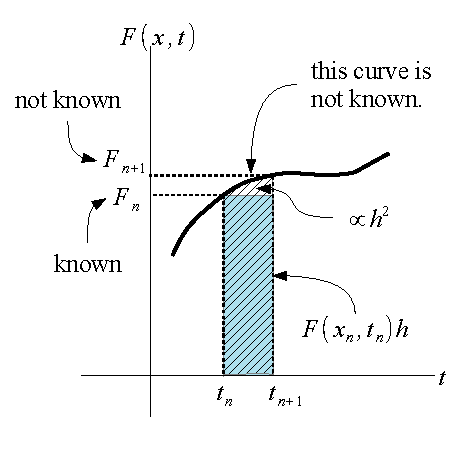
\includegraphics[width=2.5in]{05.ode1/euler-integral.pdf}
\caption{The curve in the figure represents the integrand of Eq. (\ref{eq:ode-integral}), which is unknown to us. Knowing $F_n$ and $h$, we approximate the integral by the rectangular rule.  The unaccounted area is proportional to $h^2$.}
\label{fig:euler-integral}
	\end{subfigure}
	\begin{subfigure}{0.45\textwidth}
		\centering 
		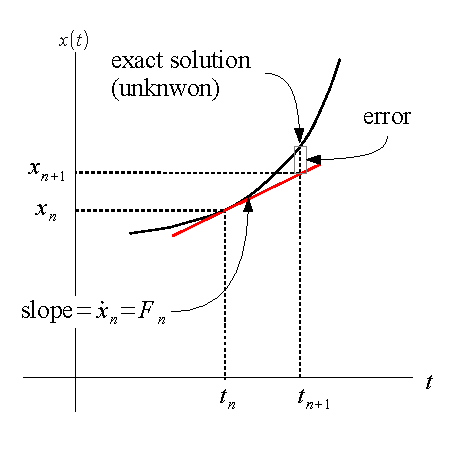
\includegraphics[width=2.5in]{05.ode1/euler-x.pdf}
\caption{Using the slope of the curve $F_n$,  we extrapolate next point $x_{n+1}$ assuming the curve is close to a straight line within a small step $h$.}
\label{fig:euler-x}
\end{subfigure}
\caption{Illustration of the Euler method}
\label{fig:euler-rule}
\end{figure}

Now, we try to estimate the integral in Eq.  \eqref{eq:ode-integral} only with known values $x_n$ and $F_n$.
Figure \ref{fig:euler-integral} shows what we are trying to do. Recalling that the rectangle rule of numerical integration depends only on the single point [see Eq. \eqref{eq:fwd-rectangle}], we use the rectangular rule to approximate the integral in Eq. \eqref{eq:ode-integral}:
\begin{equation}\label{eq:ode-rectangular}
\int_{t_n}^{t_{n+1}} F[x(t),t] \dd{t} \approx F_n\, h
\end{equation}
which leads to the Euler method:
\begin{equation}\label{eq:euler-rule}
\fbox{$x_{n+1} = x_n + F_n\, h$}.
\end{equation}


Starting from the initial value, $x_0$, we first evaluate $F_0=F(x_0,t_0)$.  Then, we obtain $x_1$ by Eq. ({eq:euler-rule}).
Using this procedure recursively, we obtain the whole sequence from $x_0$ to $x_N$.

\bigskip 
\begin{myalgobox}
	\Algorithm{Euler method}\label{algo:euler}
	
	\medskip
	\begin{minipage}{5.5in}
		\begin{enumerate}
			\item Set the total period $T$ and the number of steps $N$.
			\item Calculate the step size $h=\displaystyle\frac{T}{N}$.
			\item Set the initial condition $x_0=0$ and $t_0=0$.
			\item Reset the counter: $n=0$.
			\item Repeat the following $N$ times
			\item Evaluate the function $F_n=F(x_n,t_n)$.
			\item Calculate a new point $x_{n+1}=x_n+F_n h$.
			\item Increment the step: $n=n+1$.
			\item Go to Step 6.
		\end{enumerate}
	\end{minipage}
\end{myalgobox}
	
\bigskip
	
The area omitted in Fig. \ref{fig:euler-integral})
is order of $h^2$.  Therefore the local error of the Euler method is the order of $h^2$. After $N$ iteration, the global error becomes $N h^2 \sim \order{h}$.  If $h$ is small enough, we hope that this is a good approximation. In practice, the Euler method is not good enough for most applications.


\subsection{Predictor-Corrector Method}

The higher order of error in the Euler method  is due to the inaccuracy of the rectangle rule \eqref{eq:ode-rectangular} (See Chapter \ref{ch:integrals}).
We expect that the trapezoidal rule 
\begin{equation}\label{eq:ode-trapezoidal}
    \int_{t_n}^{t_{n+1}} F[x(t),t]\dd{t}\approx \frac{(F_n + F_{n+1}) h}{2}
\end{equation}
provides a better estimate of the integral in (\ref{eq:ode-integral}).
Then, Eq. \eqref{eq:ode-integral} becomes
\begin{equation}\label{eq:ode-implicit}
x_{n+1} = x_n + \frac{h}{2}
\left[ F(x_n,t_n) + F(x_{n+1},t_n+h) \right] + \order{h^3}.
\end{equation}
This expression is 	implicit with respect to $x_{n+1}$ since the right hand side also depends on it.
To find $x_{n+1}$, we must use a root-finding method,
which is in principle possible but too time-consuming for practical applications.  A better way is to use an approximate value of $x_{n+1}$ in the right hand side. We \emph{predict} $x_{n+1}$ using the Euler method and then \emph{correct} it by Eq. \eqref{eq:ode-implicit}.  This is the "predictor-corrector" method.  The above procedure is summarized in Algorithm \ref{algo:predictor-corrector}, which looks different from the above method but more convenient when you write a program.

\bigskip

\begin{myalgobox}
	\Algorithm{Predictor-corrector method}\label{algo:predictor-corrector}
		
	\medskip
	\begin{minipage}{5.5in}
		\begin{enumerate}
			\item Set the total period $T$ and the number of steps $N$.
			\item Calculate the step size $h=\displaystyle\frac{T}{N}$.
			\item Set the initial condition $x_0=0$ and $t_0=0$.
			\item Reset the counter: $n=0$.
			\item Repeat the following $N$ times.
			\item Increment time: $t_{n+1}=t_0 + (n+1)h$.
			\item Predictor: $k_1 = F(x_n,t_n)$						
			\item Corrector: $k_2 = F(x_n+k_1 h,t_{n+1}) $.
			\item New point: $x_{n+1}=x_n + \displaystyle\frac{h}{2} \left ( k_1 + k_2 \right )$.
			\item Increment the step: $n=n+1$.
			\item Go to Step 6.
		\end{enumerate}
	\end{minipage}
\end{myalgobox}


\bigskip
The above algorithm uses the Euler method as predictor. The local order of the error $\order{h^3}$ is better than that of the Euler method. Therefore, the corrector works.   Figure \ref{fig:predict-correct} illustrates the improvement. However, even higher accuracy can be attained if a better method such as the Adams-Bashforth method is used as predictor and a higher order corrector is used. See Ref. \cite{numerical_recipes} for the detailed description of advanced predictor-corrector methods.


\begin{figure}
	\begin{subfigure}{0.45\textwidth}
		\centering
		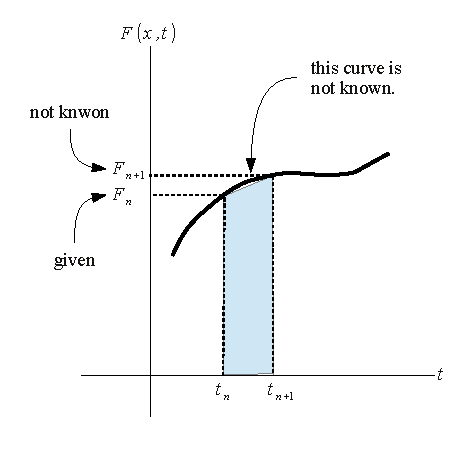
\includegraphics[height=2.5in]{05.ode1/predict-correct-integral.pdf}
\caption{$F_{n+1}$ is linearly extrapolated from two previous points $F_{n-1}$ and $F_n$.  Then, trapezoidal rule is used to integrate.}
\label{fig:predict-correct-integral}
	\end{subfigure}
	\begin{subfigure}{0.45\textwidth}
		\centering 
		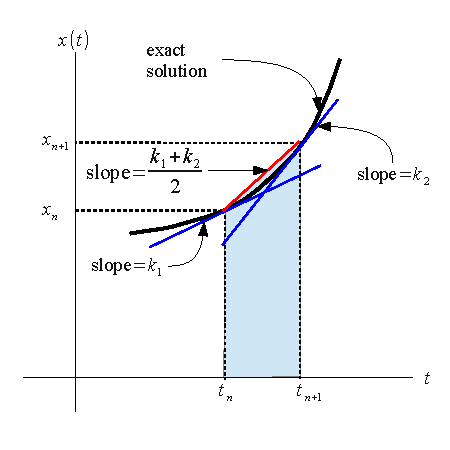
\includegraphics[height=2.5in]{05.ode1/predict-correct-x.pdf}
\caption{The linear extrapolation in the left panel is equivalent to assume that the change of the slope ($\Delta$) is the same as that in the previous step.}
\label{fig:predict-correct-rule}
	\end{subfigure}
\caption{Illustration of the Predictor-Corrector Method}\label{fig:predict-correct}
\end{figure}

\bigskip
\begin{example}[Free Falling] \label{ex:free_falling1}

\medskip
A particle of $1\, kg$ is dropped from rest in uniform gravity $9.8\, m/s^2$.  The drag force due to the presence of air is $-\gamma v$ where $v$ is velocity and the frictional coefficient is $\gamma=1.0\, kg/s$. The equation of motion is given by
\begin{equation}
m \dot{v} = - \gamma v - m g
\end{equation}
ans its solution is 
\begin{equation}
v(t) = \frac{m g}{\gamma} \left ( \me^{-\gamma t} -1 \right )\,.
\end{equation}
Let us integrate the Newton equations using Euler and Predictor-Corrector methods. Program \ref{prog:freefalling1} implements the methods.  We integrate from $t=0$ to $t=10$ using the step size $h=0.01$.  In Fig. \ref{fig:free_falling1}, the results of the two methods and the exact solution are plotted.  From naked eyes, there is no difference between them.  However, if look at the absolute errors (right panel), the difference is clear. The predictor-corrector method is much better.  Note also that the error increases at the beginning where the velocity changes very rapidly and decreases as the velocity approaches the terminal value.

\begin{figure}
\centerline{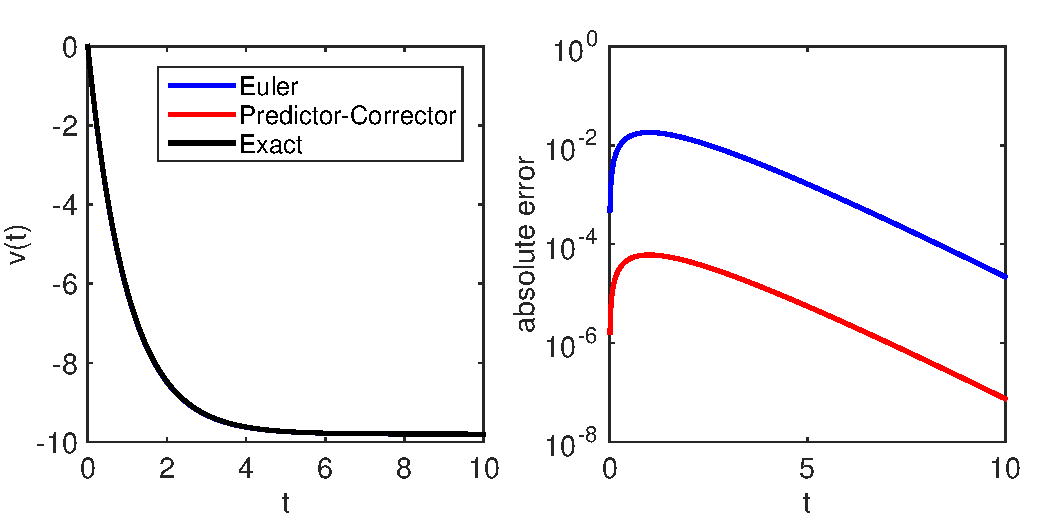
\includegraphics[height=2.5in]{05.ode1/free_falling1.pdf}}
\caption{Output of Example \ref{ex:free_falling1}.  The left panel shows the velocity as a function of time.  All three lines look identical. The right panel shows the absolute errors. The error in the predictor-corrector method is clearly  square of the error in the Euler method.}
\label{fig:free_falling1}
\end{figure}
\end{example}

\noindent
\subsection{2nd-Order Runge-Kutta Method}\label{sec:Runge-Kutta}

\begin{figure}
	\begin{subfigure}{0.45\textwidth}
		\centering
		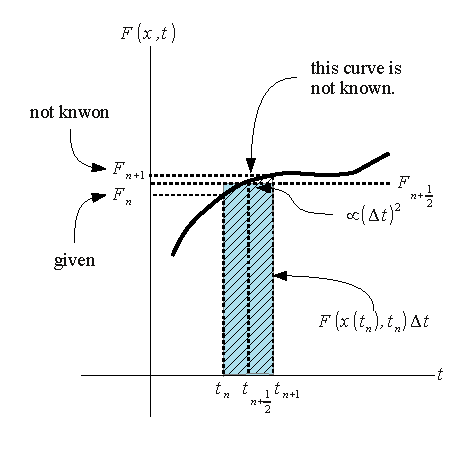
\includegraphics[height=2.5in]{05.ode1/runge-integral.pdf}
\caption{Using the Euler method, $F_{n+1/2}$ is estimated. Then, the integral is approximated by the area of the rectangle.}
\label{fig:runge-integral}
	\end{subfigure}
	\begin{subfigure}{0.45\textwidth}
		\centering 
		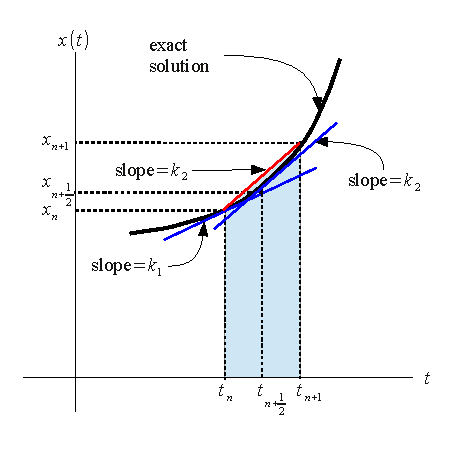
\includegraphics[height=2.5in]{05.ode1/runge-x.pdf}
\caption{The slop at the mid point ($k_2$) is estimate by the Euler method . Then the new point is predicted with the same slope (red line).}
\label{fig:runge-x}
	\end{subfigure}
\caption{Illustration of the second order Runge-Kutta Method.}
\label{fig:runge-kutta-rule}
\end{figure}

If the value of $x$ at the mid point between $x_n$ and $x_{n+1}$ 
is available, the higher
accuracy may be obtained. The integral in Eq 
\eqref{eq:ode-integral} can be evaluated by a single point (see Fig. \ref{fig:runge-kutta-rule}.):
\begin{equation}\label{eq:ode-integral-mid}
\int_{t_n}^{t_{n+1}} F(x(t),t) dt = h F_{n+1/2}.
 + \order{h^3}
\end{equation}
where $F_{n+1/2} \equiv F[]x(t_n+1/2),t_n + h/2]$, which is still unknown to us. 
We estimate it using the Euler method and obtain
\begin{equation}
x_{n+1/2} = x_n + \frac{h}{2} F_n
\label{eq:runge-mid}
\end{equation}
which enables us to compute $F_{n+1/2}$ in Eq. (\ref{eq:ode-integral-mid}). This is the second-order Runge-Kutta method. 

\bigskip
\begin{myalgobox}
	\Algorithm{Second-order Runge-Kutta method}\label{algo:runge-kutta2}

	\medskip	
	\begin{minipage}{5.5in}
		\begin{enumerate}
			\item Set the total period $T$ and the number of steps $N$.
			\item Calculate the step size $h=\displaystyle\frac{T}{N}$.
			\item Set the initial condition $x_0=0$ and $t_0=0$.
			\item Reset the counter: $n=0$.
			\item Repeat the following $N$ times.
			\item Increment time: $t_{n+1}=t_0 + (n+1)h$.
			\item Predictor: $k_1 = F(x_n,t_n)$						
			\item Corrector: $k_2 = F(x_n+k_1 h/2,t_{n}+h/2) $.
			\item New point: $x_{n+1}=x_n + k_2 h$.
			\item Increment the step: $n=n+1$.
			\item Go to Step 6.
		\end{enumerate}
	\end{minipage}
\end{myalgobox}

\bigskip

The 2nd order Runge-Kutta method has accuracy similar to the two-step Admas-Bashforth and Euler-predictor-corrector methods.
The two-step Adams-Bashforth method has a very good stability. If you need to iterate many steps, the two-step Adms-Bashforth is better than the others.
While the Runge-Kutta and the Predictor corrector methods evaluate $F$ multiple times per step, the Adams-Bashforth method evaluate it only once per step.  Therefore, the two-step Adams-Bashforth method is faster.  Therefore, if the local error $\order{h^3}$ is sufficient, the two-step Adams-Bashforth method is superior.  However, if higher accruacy is needed, the three-steps Adams-Bashforth method is not necessarily the best. The following forth-order Runge-Kutta is the winner.


\noindent
\subsection{4th-Order Runge-Kutta Method}

The Euler and two-step Adams-Bashforth methods approximate the integral in Eq. (\ref{eq:ode-integral}) using the rectangular and trapezoidal rule, respectively.  The 2nd-order Runge-Kutta is also equivalent to the trapezoidal rule.  In order to improve accuracy, it is natural to use higher order integral methods. Here we apply the Simpson rule:
\begin{equation}
\int_{x_n}^{x_{n}+h} F[]x(t),t] \dd{t} = \frac{h}{6} \left ( F_n + 4 F_{n+1/2} + F_{n+1} \right ) + \order{h^5}
\end{equation}
Since $F_{n+1/2}$ and $F_{n+1}$ are not known, we need to estimate them.  $k_2$ in the 2nd-order Runge-Kutta method is already an estimate of $F_{n+1/2}$. Now we need to estimate $F_{n+1}$ from $F_{n+1/2}$.  However, $k_2$ is based on the Euler method and not accurate enough to  predict next step.  So, we adopt the predictor-correct method to improve $F_{n+1/2}$:
\begin{equation}
k_3 \equiv  F (x_n+\frac{k_2 h}{2}, t_n+\frac{h}{2})
\end{equation}
with which we estimate the final point
\begin{equation}
k_4 \equiv F(x_n+k_3 h, t_n+h)
\end{equation}
Now both $k_2$ and $k_3$ are the estimates of $F_{n+1/2}$. Which one should we use?  In general $k_3$ should be better since the predictor-corrector method is applied. However, traditionally the mean of $k_2$ and $k_3$ is used. The local error is the order of $h^5$.  Here is the complete procedure:


\bigskip
\begin{myalgobox}
	\Algorithm{Forth-order Runge-Kutta method}\label{algo:runge-kutta4}

	\medskip			
	\begin{minipage}{5.5in}
		\begin{enumerate}
			\item Set the total period $T$ and the number of steps $N$.
			\item Calculate the step size $h=\displaystyle\frac{T}{N}$.
			\item Set the initial condition $x_0=0$ and $t_0=0$.
			\item Reset the counter: $n=0$.
			\item Repeat the following $N$ times.
			\item Increment time: $t_{n+1}=t_0 + (n+1)h$.
			\item Euler step: $k_1 = F(x_n,t_n)$			
			\item 2nd order Runge-Kutta step: $k_2 = F(x_n+k_1 h/2,t_{n}+h/2) $.
			\item Predictor-corrector step: $k_3  =  F(x_n + \frac{k_2 h}{2}, t_n + \frac{h}{2} )$.
			\item 4th order Runge-Kutta step: $k_4  =  F(x_n + k_3 h, t_n + h) $.
			\item New point: $x_n +\displaystyle\frac{h}{6} ( k_1 + 2 k_2 + 2 k_3 + k_4 )$.
			\item Increment the step: $n=n+1$.
			\item Go to Step 6.
		\end{enumerate}
	\end{minipage}
\end{myalgobox}


\bigskip
The 4th-order Runge-Kutta method is the most commonly used method in physics (or anywhere else).
Although in principle even higher order methods are possible, in practice
the fourth order is the highest that balances computing time and accuracy.

\begin{example}[Free Falling Again]\label{ex:free_falling2}  
We solve the Newton's equation in Example \ref{ex:free_falling1} using 2nd and 4th order Runge-Kutta methods.(Program \ref{prog:freefalling2})
The results shown in Fig. \ref{fig:free_falling2} indicate that the 4th order Runge-Kutta is superior.  Note also that the error of the 2nd order Runge-Kutta is essentially identical to the predictor-corrector method in Example \ref{ex:free_falling1}.
\end{example}

\begin{figure}
	\centerline{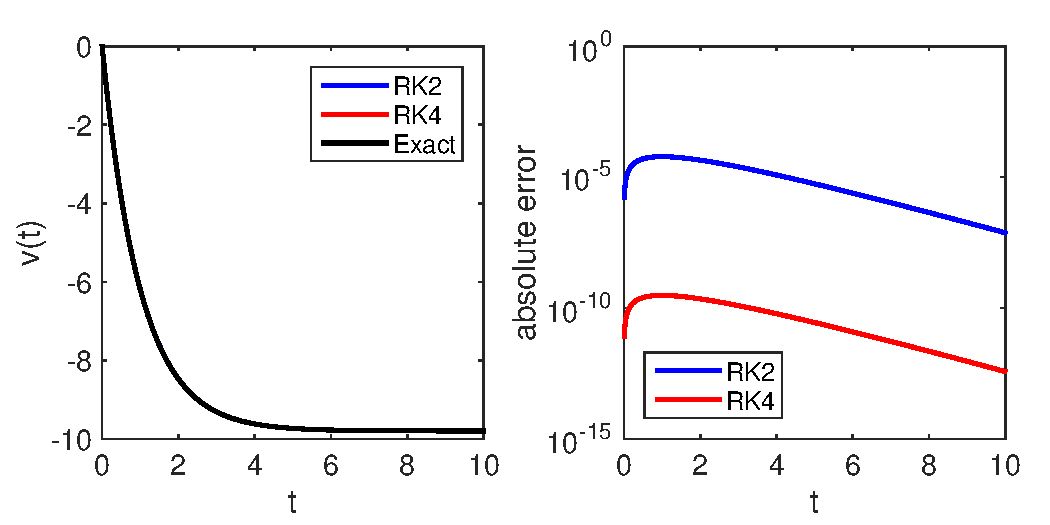
\includegraphics[height=2.5in]{05.ode1/free_falling2.pdf}}
	\caption{Output of Example \ref{ex:free_falling2}.  The left panel shows the velocity as a function of time.  All three lines look identical. The right panel shows the absolute errors. The 4th order Runge-Kutta method is clearly more accurate than the 2nd order method.}
	\label{fig:free_falling2}
\end{figure}

\noindent
\subsection{Adaptive Step: Runge-Kutta-Fehlberg Method}

The solution to an ODE can be slowly changing in some parts and rapidly varying in other parts.  If a constant step $h$ were used, it must be small enough for the rapid change.  However, such a small $h$ is not necessary in the slowly changing region and thus we waist computer time.  Furthermore, finding an appropriate step size becomes difficult if we don't know the rapidly changing part prior to the calculation.  It is desired to have an algorithm which automatically adjusts the step size as the solution is computed.  Runge-Kutta-Felberg method which is also known as RK45 finds appropriate step size so that the result is accurate to the given tolerance.

Like regular Runge-Kutta method, we try to find solution $x_{n+1}$ at $t_{n+1}$ knowing the previous step $x_n$ at $t_n$ where $t_{n+1}= t_{n}+h$.  Here we show the algorithm without proof.  For a given $h$, we evaluate the following six quantities,
\begin{subequations}
\begin{equation}
k_1 = h F(x_n,t_n)
\end{equation}
\begin{equation}
k_2 = h F\left(x_n+\frac{1}{4}k_1,t_n+\frac{1}{4}h\right)
\end{equation}
\begin{equation}
k_3 = h F\left(x_n+\frac{3}{32}k_1+\frac{9}{32}k_2,t_n+\frac{3}{8}h\right)
\end{equation}
\begin{equation}
k_4 = h F\left(x_n+\frac{1932}{2197} k_1-\frac{7200}{2197}k_2+\frac{7296}{2197}k_3,t_n+\frac{12}{13}h\right)
\end{equation}
\begin{equation}
k_5 = h F\left(x_n+\frac{439}{216} k_1 - 8 k_2 + \frac{3680}{513} k_3 - \frac{845}{4104} k_4,t_n+h \right)
\end{equation}
\begin{equation}
k_6 = h F\left(x_n -\frac{8}{27} k_1 + 2 k_2 - \frac{3544}{2565} k_3 + \frac{1859}{4104} k_4 - \frac{11}{40} k_5, t_n + \frac{1}{2} h\right)
\end{equation}
\end{subequations}
Our first try is
\begin{equation}
x_{n+1} = x_{n} + \frac{25}{216} k_1 + \frac{1408}{2565} k_3 + \frac{2197}{4101} k_4 - \frac{1}{5} k_5
\end{equation}
which uses four points ($k_1$, $k_3$, $k_4$, and $k_5$).  The second try is given by
\begin{equation}
x_{n+1}^\prime = x_{n} + \frac{16}{135} k_1 + \frac{6656}{12,825} k_3 + \frac{28,561}{56,430} k_4 - \frac{9}{
50} k_5 + \frac{2}{55} k_6.
\end{equation}
The second try is more accurate than the first try.  Now, we estimate the error by
\begin{equation}
\delta = \frac{1}{h} |x_{n+1}^\prime - x_{n+1}|.
\end{equation}
and 
\begin{equation}
\lambda = 0.84 \left ( \frac{\text{tol}}{\delta} \right )^{1/4}
\end{equation}
where tol is a tolerance.
If $\delta < \text{tol}$, then we accept the solution and move to the next step with a new step length $\lambda h$.   Since the original $h$ gives the accurate result, we want to use a larger step size.  In that case, $\lambda>1$.  If $\delta > \text{tol}$, then the present calculation is not accurate enough.  Try again with the new step size $\lambda h$ which is smaller than the original step size.  
Since the step size $h$ varies as the calculation goes, $t_n$ is no longer evenly spaced.  If we need the solution with evenly spaced $t$, we can interpolate it from the RK45 solution.

\begin{example}[Yet Another Free Falling]\label{ex:free_falling3} 
We solve the Newton's equation in Example \ref{ex:free_falling1} using Runge-Kutta-Fehlberg Method methods. MATLAB has a built-in function \texttt{ode45()} which uses the Runge-Kutta-Fehlberg algorithm. See Program \ref{prog:freefalling3}.
The result shown in Fig. \ref{fig:free_falling3} indicates that the small step size is used at the beginning and gradually increases as the magnitude of slope decreases.  The figure also shows that the error remain below the tolerance (default value in MATLAB is $10^{-3}$.).

\begin{figure}
	\centerline{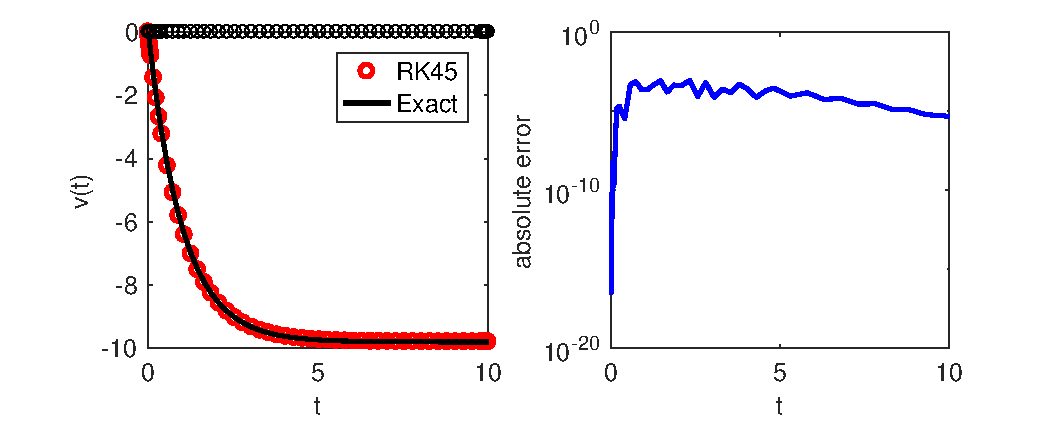
\includegraphics[height=2.5in]{05.ode1/free_falling3.pdf}}
	\caption{Output of Example \ref{ex:free_falling3}.  The left panel shows the velocity as a function of time.  The circles on the top indicates the time step.  The right panel shows the absolute errors which remains below the tolerance $10^{-3}$.}
	\label{fig:free_falling3}
\end{figure}
\end{example}
.


\noindent
\section{Coupled ODEs}

We now consider a set of ODEs. All methods we discussed in the present section can be used. Any of algorithms for single ODEs can be extended to coupled ODEs. As an example,  we solve two coupled ODEs,
\begin{subequations}
\begin{eqnarray}
\dot{x}(t) &=& F (x(t),y(t),t)\\
\dot{y}(t) &=& G (x(t),y(t),t)
\end{eqnarray}
\label{eq:coupled-ode}
\end{subequations}
using the following 4th order Runge-Kutta method:
 
\begin{subequations}
\begin{eqnarray}
&&   k_1  =  F(x_n, y_n,  t_n) \\
&&\ell_1  =  G(x_n, y_n, t_n) \\
&&   k_2  =  F(x_n + \frac{k_1 h}{2}, y_n + \frac{\ell_1 h}{2},t_n + \frac{h}{2} ) \\
&&\ell_2  =  G(x_n + \frac{k_1 h}{2}, y_n + \frac{\ell_1 h}{2},t_n + \frac{h}{2} ) \\
&&   k_3  =  F(x_n + \frac{k_2 h}{2}, y_n + \frac{\ell_2 h}{2},t_n + \frac{h}{2} ) \\
&&\ell_3  =  G(x_n + \frac{k_2 h}{2}, y_n + \frac{\ell_2 h}{2},t_n + \frac{h}{2} ) \\
&&   k_4  =  F(x_n + k_3 h, y_n + \ell_3 h, t_n + h) \\
&&\ell_4  =  G(x_n + k_3 h, y_n + \ell_3 h, t_n + h) \\
&&x_{n+1}  =  x_n +\displaystyle\frac{h}{6} ( k_1 + 2 k_2 + 2 k_3 + k_4 )\\
&&y_{n+1}  =  y_n +\displaystyle\frac{h}{6} ( \ell_1 + 2 \ell_2 + 2 \ell_3 + \ell_4 )
\end{eqnarray}
\end{subequations}


\begin{example}[Two Cars]\label{ex:twocars}
Two cars  move with velocity $v_1$ and $v_2$.  The driver of each car tries to keep its velocity the same as the velocity of other car. Using a simple linear coupling between two cars, their equations of motion are model as
\begin{eqnarray}
\dot{v}_1 &=& + k (v_2-v_1) \nonumber \\
\dot{v}_2 &=& - k (v_2-v_1)
\end{eqnarray}
where $k$ is a positive constant.  By adjusting the unit of time, we can set $k=1$.  Initially, the first car was slightly faster than the second: $v_1(0) = 1.2$ and $v_2(0) = 1.0$.  Are they able to travel together? If so, how soon their speed is synchronized?  What is their final velocity?  Since the equation is linear, this problem can be solved analytically.  The answer is "yes".  The velocity difference decays as $\delta v = \delta v_0 \me^{-2t}$ and the final velocity is the mean of the initial velocities $v_f = \frac{1}{2} (v_1(0)+v_2(0))$.  Here we solve the equations using the 2nd-order Runge-Kutta and the results are plotted in Fig. \ref{fig:twocars}.

\begin{figure}
\centerline{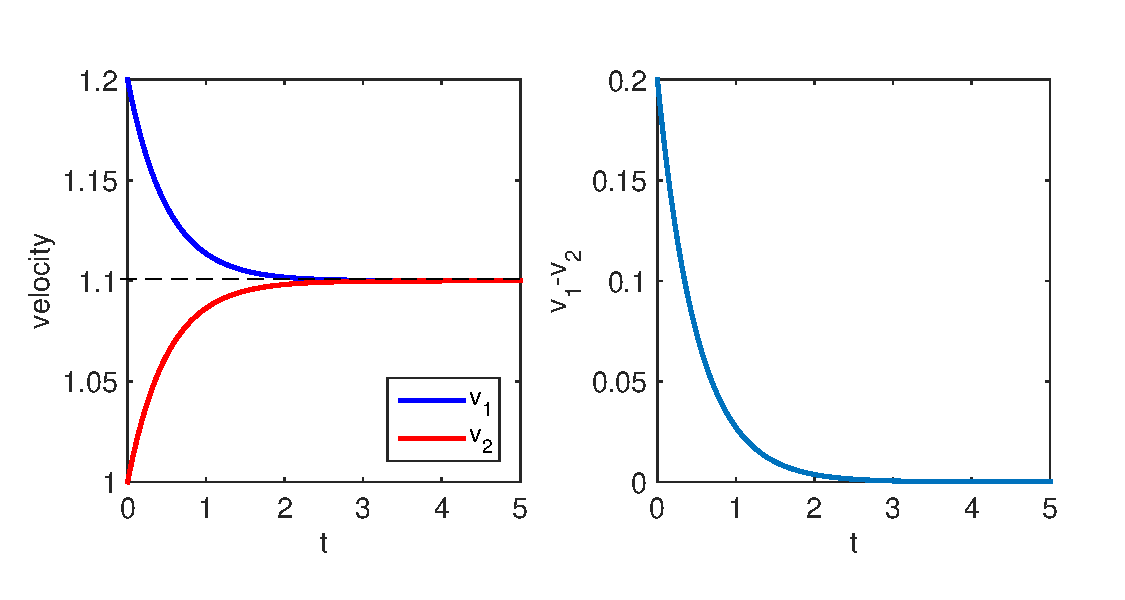
\includegraphics[height=2.5in]{05.ode1/twocars.pdf}}
\caption{Output of Example \ref{ex:twocars}.  Left: The velocity of each car. At the end two cars travel at the same velocity. Right: The difference in velocities.  The velocity difference decreases exponentially. The 2nd order Runge-Kutta method with $h=0.02$ is used.}
\label{fig:twocars}
\end{figure}
\end{example}



\section{Second-Order Differential Equations}

Many second-order ODEs in physics problems can be converted to a set of coupled first-order ODEs.  The methods discussed in the previous sections can be used to solve them without any additional steps.  On the other hand, there are algorithms specifically developed for second-order ODEs such as Newton's equations of motion.  

\subsection{Converting to a Coupled First-Order ODEs}
Consider a second-order differential equation
\begin{equation}
\ddot{x} = F(x,\dot{x},t).
\label{eq:ode2nd}
\end{equation}
Introducing a new variable $y = \dot{x}$, Eq (\ref{eq:ode2nd}) can be written as
a set of coupled first-order differential equations,
\begin{eqnarray}
\dot{y} & = & F(x,y,t) \\
\dot{x} & = & y ,
\end{eqnarray}
which can be solved by the method discussed in the previous section.


Newton's equation of motion are this type of ODEs.  For more complicated classical systems, Lagrangian approach is often used. Euler-Lagrange equations generate the second order ODEs which can be transformed to this type. If the system is conservative, Hamiltonian approach may be more convenient for numerical methods since the Hamilton's canonical equations of motion are already a set of first order ODEs.


\bigskip

\begin{example}[Simple Harmonic Oscillator]\label{ex:harmonic_oscillator1}  
A harmonic oscillator of mass $m$ and spring constant $k$ oscillates with frequency $\omega=\sqrt{\frac{k}{m}}$.  The dynamics is determined by the Newton's equation of motion
\begin{equation}
m \ddot{x} = - k x  \quad \rightarrow \quad \ddot{x} = -\omega^2 x\, .
\end{equation}
First, we convert it to coupled ODEs
\begin{subequations}
\begin{eqnarray}
\dot{v} &=& - \omega^2 x \\
\dot{x} &=& v
\end{eqnarray}
\end{subequations}
and solve it with the 4th-order Runge-Kutta method. Figure \ref{fig:harmonic_oscillator1} illustrates the accuracy of the method.  Note that the error gradually increases as the number of iterations increases.

\begin{figure}
\centerline{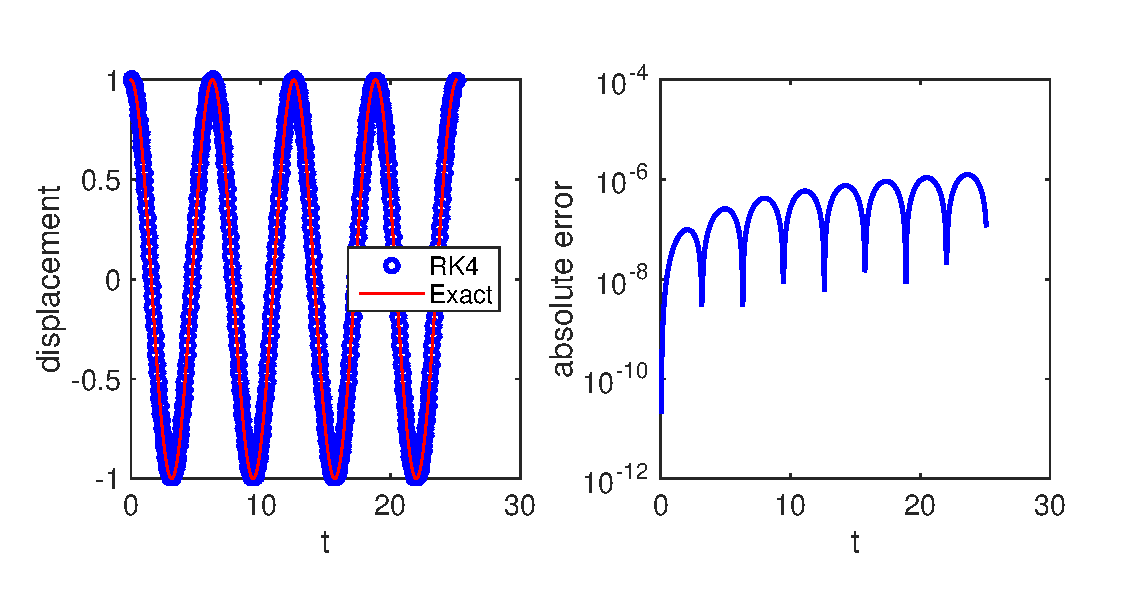
\includegraphics[height=2.5in]{05.ode1/harmonic_oscillator1.pdf}}
\caption{Left: Trajectory of a simple harmonic oscillator ($\omega=1$): The Newtons equation of motion is integrated with 4th order Runge-Kutta method ($h=0.05$).  Right: Absolute error. The error is very small but gradually increasing as the number of iterations increase. }
\label{fig:harmonic_oscillator1}
\end{figure}

\exercise
Add the friction term $-gamma \dot{x}$ in the program.  Plot trajectories for $\gamma^2 > 4 m k$ (weakly damped), $\gamma^2=4 m k$ (critically damped), and $\gamma^2 < 4 m k$ (overdamped).
\end{example}


\noindent
\subsection{Verlet Method}

\smallskip
Although any second order differential equation can be rewritten as
a coupled first-order differential equation, there are convenient
methods that directly solves second-order differential equations.
However, these methods works only for certain types of
second-order equations.  Newton equations,
\begin{equation}
\ddot{x} = \frac{1}{m} F(x,t)
\label{eq:newton}
\end{equation}
is an example.  Note that the force does not depend on velocity.

Using the Taylor expansion,
\begin{eqnarray}
x(t+h) & = & x(t) + h \dot{x}
 + \frac{h^2}{2} \ddot{x} + \frac{h^3}{6} x^{(3)}
 + O(h^4) \\
x(t-h) & = & x(t) - h \dot{x}
 + \frac{h^2}{2}\ddot{x} - \frac{h^3}{6} x^{(3)}
 + O(h^4) 
\end{eqnarray}
Adding these equations cancels the odd-order terms and we obtain
\begin{eqnarray}
x(t+h) & = & 2 x(t) - x(t-h) + h^2 \ddot{x} + O(h^4) \\
       & = & 2 x(t) - x(t-h) + \frac{h^2}{m} F(x(t),t) + o(h^4)
\end{eqnarray}
which leads to a recursive equation
\begin{equation}
\fbox{$x_{n+1} = 2 x_n - x_{n-1} + F_n \frac{h^2}{m} + o(h^4)$}
\end{equation}
This simple iteration scheme gives rise to the accuracy of $o(h^4)$, only one order worse than the 4th-order Runge-Kutta. This simplicity is due to the fact that the force does not depend
on the velocity. Since the velocity-dependent force such as friction does not appear in microscopic picture, this method is widely used in the molecular dynamics simulation.  We need to consider not only the degree of error but also the computation time.  The Verlet method evaluates the force only once in each step whereas the 4th-order Runge-Kutta needs to evaluate it four times.  Therefore, the Verlet method is more suitable for large scale simulation.

One problem is that this recursive equation uses two previous steps.  However, the given initial condition is
$x_0$ and $v_0$.  In order to find $x_1$ we need to know $x_{-1}$!   A popular resolution is to use Euler method only for the first step.
\begin{equation}
x_{1} = x_0 + v_0 h + F_0 \frac{h^2}{m}\, .
\end{equation}

The velocity can be obtained by the mean value 
numerical derivative:
\begin{equation}
v_n = \dot{x}_n = \frac{x_{n+1} - x_{n-1}}{2h}
\end{equation}




\bigskip
\begin{example}[Simple harmonic oscillator again]\label{eq:harmonic_oscillator2} 
We repeat Example \ref{ex:harmonic_oscillator1} but with the Verlet method (Program \ref{prog:harmonic_oscillator2})  The result indicates that the error is larger than that of the 4th-order Runge-Kutta as expected.  However, for many large simulation, the degree of accuracy is good enough.

\begin{figure}
\centerline{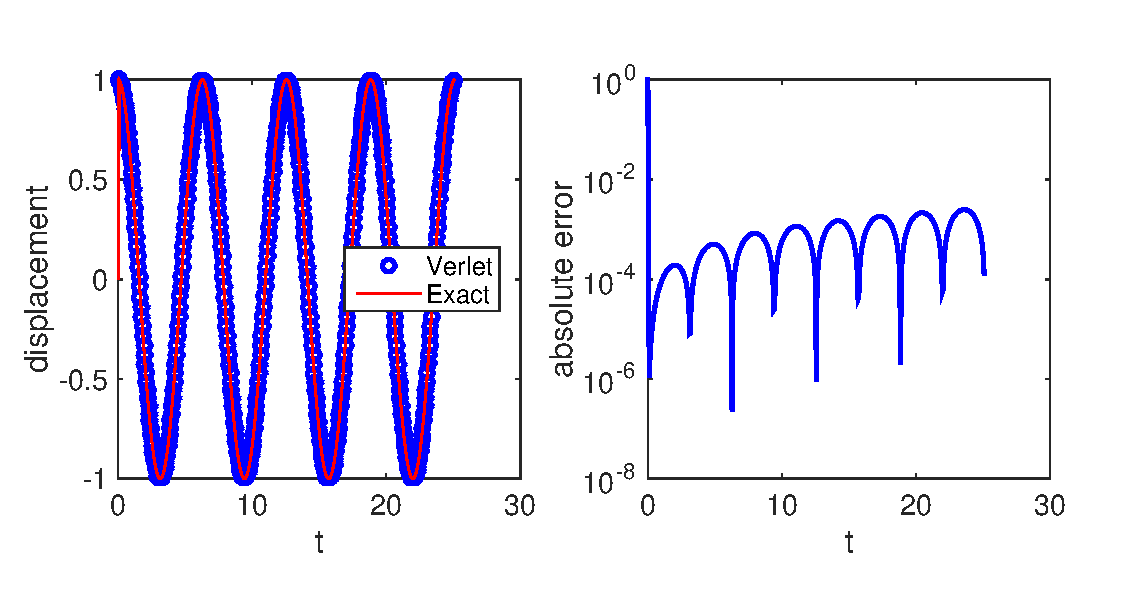
\includegraphics[height=2.5in]{05.ode1/harmonic_oscillator2.pdf}}
\caption{Left: Trajectory of a simple harmonic oscillator ($\omega=1$): The Newtons equation of motion is integrated with Verlet method ($h=0.05$).  Right: Absolute error. The error is small but considerably larger that of 4th-order Runge-Kutta method in Fig. \ref{fig:harmonic_oscillator1}. }
\label{fig:harmonic_oscillator2}
\end{figure}

\exercise
Consider a forced harmonic oscillator with external forcing $A \cos(\Omega t)$ where $A$ and $\Omega$ are amplitude and frequency of the external force.  Calculate trajectories of the forced oscillator using the Verlet method.
\end{example}

\section{Applications in Physics}

\subsection{Nonlinear Chemical Dynamics: Brusselator}

\begin{figure}
\centerline{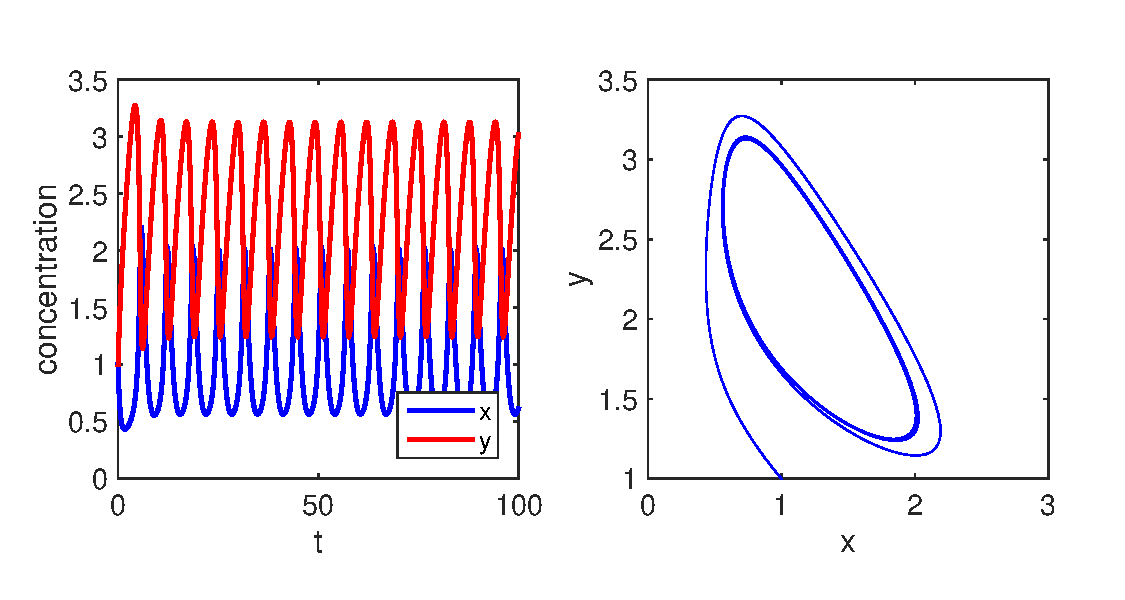
\includegraphics[height=2.5in]{05.ode1/brusselator.pdf}}
\caption{Limit cycle in the Brusselator dynamics. Parameter values: $a=1$ and $b=2.3$}
\label{fig:brusselator}
\end{figure}

\noindent
In order to investigate self-organization mechanisms, the following hypothetical chemical reaction (Brusselator model) has been intensively investigated:
\begin{absolutelynopagebreak}
\begin{subequations}\label{eq:reaction}
\begin{equation}
A \longrightarrow X \\ 
\end{equation}
\begin{equation}
B + X \longrightarrow Y + D
\end{equation}
\begin{equation}
2X + Y \longrightarrow 3X
\end{equation}
\begin{equation}
X \longrightarrow E
\end{equation}
\end{subequations}
\end{absolutelynopagebreak}
\noindent
where the species $A$ and $B$ are sources injected into the system such that their concentration is kept
constant, and the products $D$ and $E$ are extracted from the system at a
constant rate. The species $X$ and $Y$ are intermediate products. 
It is important to note that both $X$ and $Y$ are produced and
consumed during the sequence of reactions in such a way that $X$
produces $Y$ and in turn $Y$ produces $X$.

Corresponding to the chemical equations (\ref{eq:reaction}), the time
evolution of the concentration of $X$ and $Y$ in the Brusselator system is determined by
coupled differential equations:
\begin{subequations}
\label{eq:brusselator}
\begin{equation}
\dot{x} = a-(b+1)x + x^2 y
\end{equation}
\begin{equation}
\dot{y} = bx - x^2 y
\end{equation}
\end{subequations}
where $a$ and $b$ are the concentration of $A$ and $B$ in the Brusselator
model (\ref{eq:reaction}) which are control parameters, and
$x$ and $y$ are the concentration of $X$ and $Y$  In Program \ref{prog:brusselator} the differential equations is integrated with the 4th-order Runge-Kutta method.  Initial conditions
$x_0=1$ and $y_0$=1 and parameter values $a=1$ and $1.5<b<2.5$ are used. As $b$ is varied the type of trajectories changes (bifurcation). 
In an interesting case, the solution converges to a closed loop regardless of the initial condition. This kind of dynamics is known as limit cycle.\cite{brusselator} and plays important roles in biological systems.\cite{limitcycle1,limitcycle2} Figure \ref{fig:brusselator} illustrates the limit cycle obtained by Program \ref{prog:brusselator} with parameter values $a=1$ and $b=2.3$.


\subsection{Nonlinear Dynamics in Laser: Maxwell-Bloch equation}\label{sec:maxwell_bloch}

\medskip\noindent
A semiclassical model of the laser is known as Maxwell-Bloch equation\cite{chaos1,chaos2}:
\begin{subequations}\label{eq:maxwell-bloch}
	\begin{equation}
	\dot{E} = - \gamma_1 E + \kappa_1 P 
	\end{equation}
	\begin{equation}
	\dot{P} = - \gamma_2 P + \kappa_2 E\, D
	\end{equation}
	\begin{equation}
	\dot{D} = - \gamma_3 (D-\lambda) - \kappa_3 E\, P
	\end{equation}
\end{subequations}
\noindent
where $E$, $P$, $D$ are the electric field, the mean polarization of atoms, and the population inversion, respectively.
$\gamma_1$ are the decay rates of the electric field in the laser cavity due to beam transmission.  $\gamma_2$ and $\gamma_3$ are the decay rates of the atomic polarization and population inversion, respectively. $\kappa_i, i=1,2,3$ are positive coupling constants.  $\lambda$ is the energy pumping parameter and may be positive, negative or zero.  Unlike two-dimensional nonlinear dynamics of the Brusselator model, this is three-dimensional nonlinear dynamics and chaotic trajectories are possible. Depending on the parameter values, the system shows a variety of dynamics. We solve the coupled ODEs using 2nd-order Runge-Kutta method from $t=0$ to $t=500$ (or longer) for each parameter set given in Table \ref{tbl:maxwell_bloch}. Then, we investigate the time evolution of $E$ and two-dimensional phase trajectory ($E$, $D$) for each of  the following cases. Type C shows a particularly interesting trajectory known as \emph{strange atractor} which is confined in a finite region without repeating itself as shown in Fig. \ref{fig:maxwell_bloch}.  Such a trajectory is possible only in three or higher dimensional phase spaces.

\begin{center}
\begin{minipage}{5.5in}  
\begin{itemize}
\item [Type A] Vary $\lambda$ from 3.0 to 6.0.  Observe that $E$ always converges to a constant value.  However, below a certain critical value of $\lambda$, $E$ decays to zero.  On the other hand, above it $E$ goes to a positive vale (lasing).
\item [Type B] Vary $\lambda$ from 0.5 to 3. Observe that $E$ always converges to a constant value.  However, below a certain critical value of $\lambda$, $E$ decays to zero.  On the other hand, above it $E$ goes to a positive vale (lasing).
\item [Type C] Vary $\lambda$ from 20 to 25. Observe that $E$ decays to zero with oscillation below a critical value of $\lambda$.  Above the critical value, $E$ randomly oscillates (unstable laser).
\end{itemize}
\end{minipage}
\end{center}

 
\begin{table}[t]
\begin{center}
\footnotesize
\begin{tabular}{c|llllll}
\hline
Type & $\gamma_1$ & $\gamma_2$ & $\gamma_3$ & $\kappa_1$ & $\kappa_2$ & $\kappa_3$ \\
\hline
A ($\gamma_2, \gamma_3 \gg \gamma_1$) & 0.1 & 2 & 3 & 0.25 & 0.2 & 1\\
B ($\gamma_2 \gg \gamma_1, \gamma_3$) & 0.1 & 10 & 0.25 & 1 & 0.5 & 1\\
C ($\gamma_1 > \gamma_2 + \gamma_3$)  & 1 & 0.1 & 0.25 & 1 & 0.1 & 1\\
\hline
\end{tabular}
\end{center}
\caption{Parameter sets for Maxwell-Bloch equation.}\label{tbl:maxwell_bloch}
\end{table}

\begin{figure}
\center
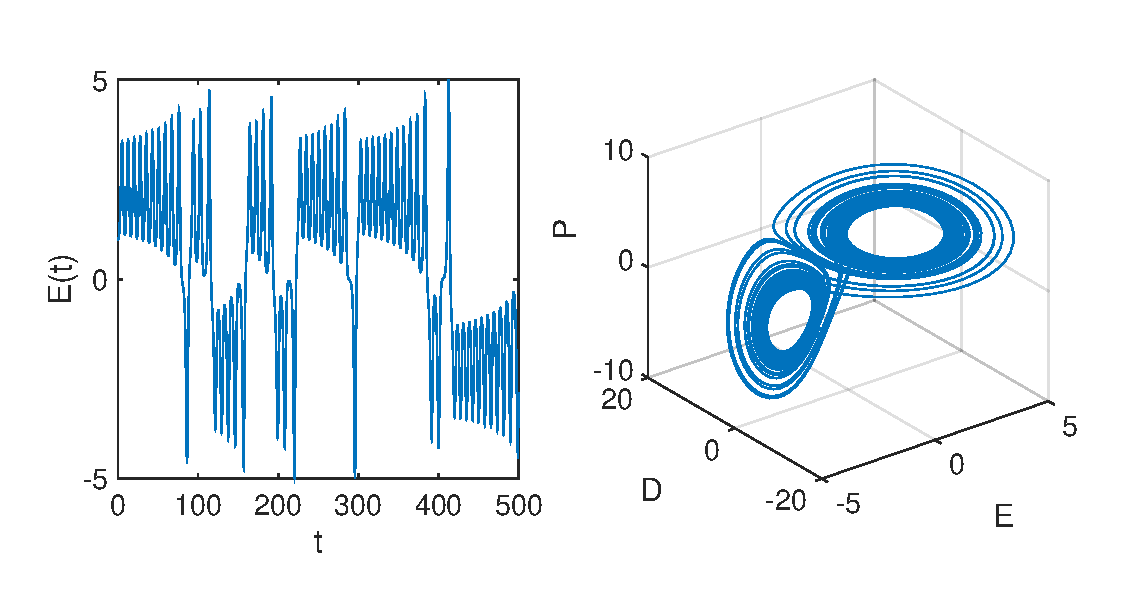
\includegraphics[height=2.5in]{05.ode1/maxwell_bloch.pdf}
\caption{Left: Erroneous oscillation in the magnitude of electric field. Right: Three--dimensional phase plot of $E$, $P$ and $D$ showing a strange attractor.  Parameter values: Type C in Table \ref{tbl:maxwell_bloch} and $\lambda=23$}
\label{fig:maxwell_bloch}
\end{figure}

\subsection{Frequency Entrainment and Phase Synchronization}

Rhythmical oscillations are ubiquitous phenomena such as heart beat, burst of neuron, circadian rhythm and hands clapping.  Each oscillation has its own frequency, phase, and amplitude.  Consider a large number of oscillators interacting each other.  Each oscillator has a slightly different frequency and phase from each others. With an appropriate interaction, the all oscillators begin  oscillating in unison with the identical frequency and the same phase despite that individual oscillators have different natural frequencies. This is the phenomenon of synchronization.\cite{sync} For example imagine hand clapping at the end of a ballet performance.  At the beginning, the clapping is not unison but soon everyone is clapping at the same frequency and phase with others.  Most spectacular phenomenon is simultaneous flashing of thousands of fireflies in Southeast Asia.\cite{sync,fireflies}  An example in physics is synchronization of the array of Josephson junctions.\cite{sync}

We investigate a similar phenomena using the Kuramoto model.
The dynamics of phase variables $\theta_1$ and $\theta_2$ is described by a coupled ODEs\cite{coupled_oscillators}:
\begin{subequations}
\begin{eqnarray}
\dot{\theta_1}&=& \omega_1 + \sin(\theta_2-\theta_1)\\
\dot{\theta_2}&=& \omega_2 - \sin(\theta_2-\theta_1)
\end{eqnarray}
\label{eq:kuramoto}
\end{subequations}
\noindent
where $\omega_1$ and $\omega_2$ are natural frequencies of the individual phase oscillator.  When there is no coupling, each oscillator oscillates with its own frequency.
This problem is similar to the two car problem (Example \ref{ex:twocars}).  However, the coupling is now nonlinear and more dramatic phenomena such as phase entrainment and synchronization can be seen in this model.
Program \ref{prog:kuramoto} integrates Eq. (\ref{eq:kuramoto}) with the 2nd-order Runge-Kutta method.  The results are plotted in Fig.
\ref{fig:kuramoto}.   Initially the oscillators are in different phases and periods.  Despite of their different natural frequencies, they oscillates in the exactly the same period (frequency entrainment) and with a constant phase difference (phase synchronization).

\begin{figure}
\centerline{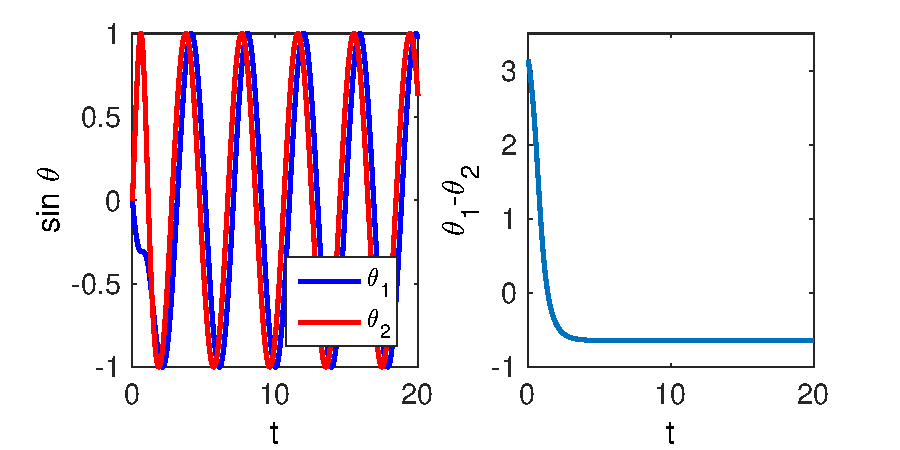
\includegraphics[height=2.5in]{05.ode1/kuramoto.pdf}}
\caption{Left: The trajectory of the oscillators.  Each oscillator has its own natural frequency $\omega_1=1.0$ and $\omega_2=1.2$. Initially the two oscillators are out of phase.  Despite of these differences, they are quickly synchronized  and oscillate at the same frequency. Left: the phase difference rapidly changes at the beginning but settles to a constant phase difference.  [The 2nd-order Runge-Kutta is used with $h=0.01$.]}
\label{fig:kuramoto}
\end{figure}

\bigskip
\exercise
Observe that for $\omega_1=1.0$ and $\omega_2=2.2$, frequency entrainment still takes place.  However, the phase difference no longer vanishes.

\exercise
Observe that for $\omega_1=1.0$ and $\omega_2=3.2$, neither frequency entrainment nor phase synchronization occur.  The difference between the two oscillators is too big,


\subsection{Period of Oscillation}

In Sec \ref{sec:oscillation1}, 
we discussed how to evaluate the analytical expression of the period of oscillation using numerical integration.  Here we simulate the oscillation by solving the Newton's equation of motion numerically.  We assume that the analytical form of the force,
$F(x) = - U'(x)$, is known. You can pick any initial condition consistent with the given energy $E$. For example, the initial position $x_0$ is chosen somewhere  between two turning points. The initial velocity is then determined by the energy conservation law
%
\begin{equation}
\frac{m}{2} v_0^2 + U(x_0) = E \quad \rightarrow \quad v_0 = \pm \sqrt{\frac{2 (E-U(x_0))}{m}}
\end{equation}
%
The sign determines the direction of initial velocity.

To determine the period of oscillation, we measure the time the particle comes back to the starting point.  To increase accuracy, we measure the time $\tau$ the particle returns to the starting point after $N$ oscillations.  Then, the period is $T=\tau/N$. One problem is that the time is discrete and we don't know the exact time the particle returned.  Suppose that the particle passes the initial position between $t_n$ and $t_{n+1}$. That means $t_n < \tau <t_{n+1}$ and $x_{n} < x_0 < x_{n+1}$ (assuming that the direction of the initial velocity is positive.)  
Using the Euler method, the time to reach the starting point is $\tau = t_n + \delta$ where $delat$ is a positive solution of quadratic equation
\begin{equation}
x_0 = x_{n} + v_{n} \delta + F_{n} \frac{\delta^2}{2 m}
\end{equation}
for $\delta=t_{n+1}-\tau$.  Choosing the smaller root, the answer is
\begin{equation}
\delta = \frac{ -v_{n} \pm \sqrt{v_{n}^2 - 2 (x_n-x_0) F_{n}/m}}{F_n/m}
\end{equation}
One of the solutions are positive depending on the sign of the force $F_n$.
Since $x_n-x_0$ may be very small, we need to take care of the bit-off error discussed in Problem 1.1. 
Program \ref{prog:period} evaluates the period of simple harmonic oscillator (see Example \ref{ex:harmonic_oscillator1}) using the Verlet method. With $h=0.05$, the Verlet method predicts $T=6.283159$, in a good agreement with the exact answer $T=2\pi$. 



\subsection{Pendulum}

\begin{figure}
\centerline{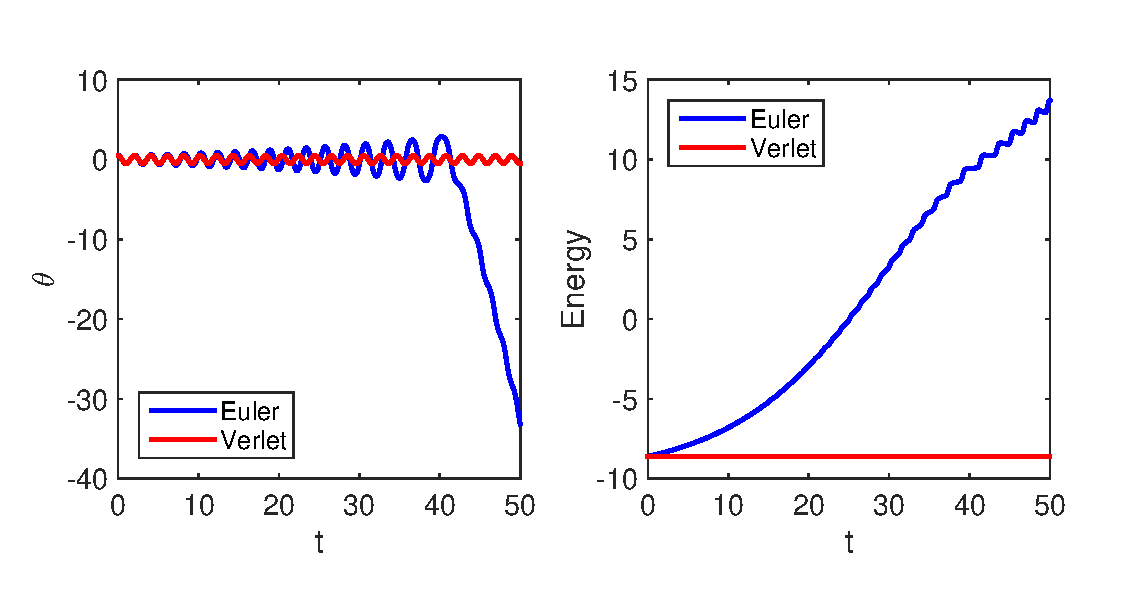
\includegraphics[height=2.5in]{05.ode1/pendulum_instability.pdf}}
\caption{The numerical instability with the Euler method.  Left: Time evolution of angular coordinate $\theta$. The result of the Verlet method oscillates periodically as expected. However, the output of the Euler method oscillates with increasing amplitude and diverges at the end. Right: Mechanical energy.  The energy with the Verlet method conserves but that of the Euler method keeps increasing. Integration step size $h=0.01$ is used.}
\label{fig:pendulum_instability}
\end{figure}

A pendulum consisting of a bob of mass $m$ and a massless rod of length $\ell$ exhibits two types of motion, oscillation around a stable equilibrium and rotation in one way.
Using the angular coordinate, the equation of motion of a simple pendulum is
\begin{equation}
I \ddot{\theta} = - m g \ell \sin \theta
\end{equation}
where $I=m \ell^2$ is the moment of inertia.  Simplifying the equation,
\begin{equation}
\ddot{\theta} = -\Omega^2 \sin \theta
\end{equation}
where $\Omega = \sqrt{\displaystyle\frac{g}{\ell}}$. Let integrate this equation using two different methods, Euler and Verlet methods.  We are not only interested in the coordinate but also the mechanical energy
\begin{equation}
E=\frac{I \omega^2}{2} - m g \ell \cos\theta
\end{equation}
where $\omega=\dot{\theta}$ is angular velocity.
For simplicity, we use parameter values $m=1\, kg$ and $\ell=1\, m$.  The gravity is $g=9.8\, m/s^2$.  We start the motion as
$\theta_0 = 0.5$ rad and $\omega_0=0$. We expect the oscillatory motion. Figure \ref{fig:pendulum_instability} shows clearly unrealistic trajectory. Using the time step $h=0.01$, the Euler method predicts monotonic increase in the amplitude of oscillation and rotational motion begins after a certain time. The energy monotonically increases in violation of the energy conservation law.  It is clear that the Euler method keeps moving away from the exact solution. This kind of behavior is called numerical instability. The Verlet method , on the other hand, correctly predicts periodic oscillation and constant energy.

\bigskip
\exercise
Does the Euler method produce a resonable trajectory with a smaller $h$, say $h=0.001$? 

\subsection{Scattering Angle}

In Sec. 2.3.2, % \ref{sec:scattering1}
the scattering angle is given as an improper integral which we integrated numerically.  Here, we directly integrate the Newton's equation and compare the results with the previous results.  Due to the conservation of momentum, the motion is confined in a plane determined by the velocity and position vectors.  Therefore, we consider trajectories only on the $xy$ plane where $x$ is the direction of the initial velocity.  The potential is 
\begin{equation}\label{eq:scattering_potential2}
U(x,y) = \frac{k}{r} \me^{-r/a}
\end{equation}
where $r=\sqrt{x^2+y^2}$.
The corresponding force on the particle is 
\begin{subequations}
\begin{eqnarray}
F_x &=& -\frac{\md}{\md x} U(x,y) = \frac{k x}{r^2} \left ( \frac{1}{r}+\frac{1}{a} \right ) \me^{-r/a}\\
F_y &=& -\frac{\md}{\md y} U(x,y) = \frac{k y}{r^2} \left ( \frac{1}{r}+\frac{1}{a} \right ) \me^{-r/a}
\end{eqnarray}
\end{subequations}
Using $\sqrt{{m a^3}/{k}}$ and $a$ as units of time and distance, respectively, 
the equations of motion becomes free of parameters as 
\begin{subequations}
\begin{eqnarray}
\ddot{x} &=& \frac{x}{r^2} \left ( \frac{1}{r}+1 \right ) \me^{-r}\\
\ddot{y} &=& \frac{y}{r^2} \left ( \frac{1}{r}+1 \right ) \me^{-r}
\end{eqnarray}
\end{subequations}
In this units, the energy is measured in $k/a$.
Now, we need to specify the initial conditions.  Assuming that the particle is impinged along $x$ axis with impact parameter $b$,
$x_0=-10$, $y_0=b$, $v_{y0}=0$, and $v_{x0}=\sqrt{2E}$.   The impact parameter $b$ and energy $E$ uniquely determine the trajectory.

Since the force does not depend on the velocity, the Verlet method can be used to integrate the coupled ODE.
When the particle leaves the scattering region (say, $r>10$), we stop the integration.  Program \ref{prog:scattering2} solves the Newton equation and calculates the scattering angle
\begin{equation}
\theta =\cos^{-1} (\mathbf{v_0}\cdot \mathbf{v_f}/v_0 v_f) = \cos^{-1} (\mathbf{v_0}\cdot \mathbf{v_f}/2E)
\end{equation}
where $\mathbf{v_f}$ is the final velocity.  Since energy conserves $v_0 v_f = v_0^2 = 2E$.

The left panel of Fig. \ref{fig:scattering2} shows several trajectories with different impact parameters forming a shadow cone behind the target.  The right panel plots the scattering angle as a function of impact parameter.

\begin{figure}
\centerline{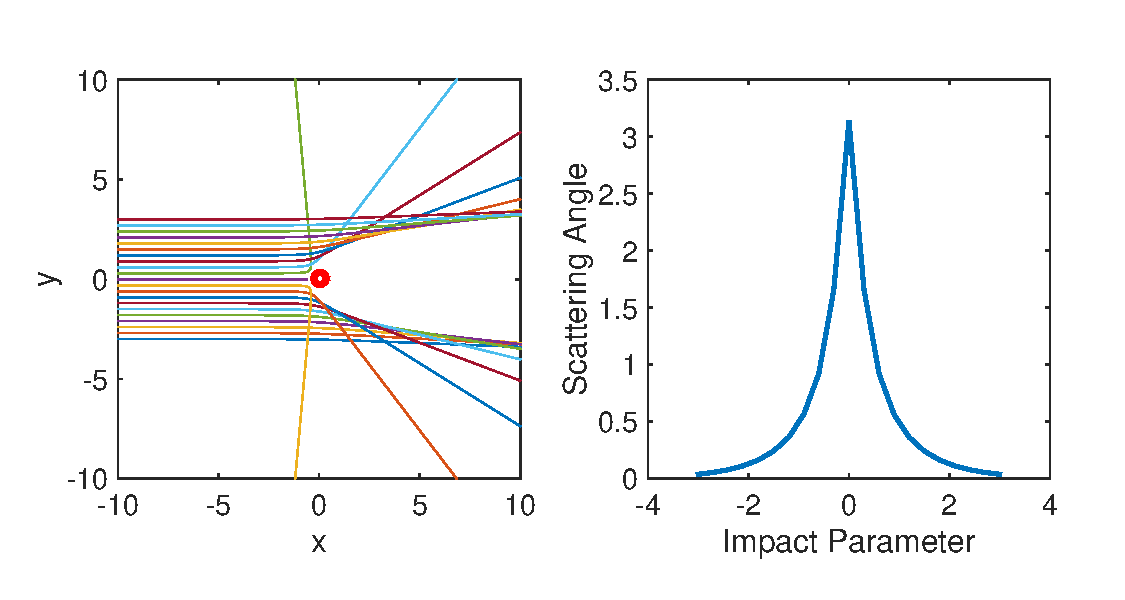
\includegraphics[height=2.5in]{05.ode1/scattering2.pdf}}
\caption{Scattering by a screened Coulomb force. Left: trajectories with different impact parameters. Notice the shadow cone behind the target where the particle cannot enter.  Right: Scattering angle $\theta$ determined by the simulation.}
\label{fig:scattering2}
\end{figure}

\bigskip
\exercise
Calculate the trajectories and scattering angle for $k<0$.

\subsection{Double Pendulum}


A double pendulum is a popular example in classical mechanics courses.  The Lagrangian approach beautifully derives the equations of motion:
\begin{subequations}\label{eq:double_pendulum}
\begin{eqnarray}
&& \begin{aligned}
(m_1+m_2) L_1 \ddot{\theta}_1 &+ m_2 L_2 \ddot{\theta}_2 \cos(\theta_1-\theta_2) + m_2 L_2 \dot{\theta}_2^2 \sin(\theta_1-\theta_2)\\
& + (m_1+m_2) g \sin \theta_1 = 0 
\end{aligned}\\
&&
m_2 L_1\ddot{\theta}_1 \cos(\theta_1-\theta_2) + m_2 L_2 \ddot{\theta}_2 - m_2 L_1\dot{\theta}_1^2 \sin(\theta_1-\theta_2)
+ m_2 g \sin \theta_2 = 0
\end{eqnarray}
\end{subequations}
\normalsize
where the angular coordinates $\theta_1$ and $\theta_2$ are defined in Fig.  \ref{fig:double_pendulum}.
These equations of motion are awfully complicated and there is little hope to find an analytical solution. Thus we resort to a numerical method.  Since Eqs (\ref{eq:double_pendulum}) contains both $\ddot{\theta}_1$ and $\ddot{\theta}_2$, standard numerical methods cannot be applied.  They must be rewritten in such a way that a standard numerical method can be applied.  After complicated algebra, we find
\begin{subequations}
\begin{eqnarray}
\dot{\omega}_1 &=& \frac{D E - B F}{A D - B C}\\
\dot{\omega}_2 &=& \frac{A F - C E}{A D - B C}\\
\dot{\theta}_1 &=& \omega_1\\
\dot{\theta}_2 &=& \omega_2
\end{eqnarray}\\
\label{eq:double_pendulum2}
\end{subequations}
where
\begin{subequations}
\begin{eqnarray}
A &=& (m_1+m_2) L_1 \\
B &=& m_2 L_2 \cos(\theta_1 - \theta_2)\\
C &=& m_2 L_1 \cos(\theta_1 - \theta_2) \\
D &=& m_2 L_2 \\
E &=& - m_2 L_2 \omega_2^2 \sin(\theta_1-\theta_2) - (m_1+m_2) g \sin\theta_1\\
F &=& m_2 L_1 \omega_1^2 \sin(\theta_1-\theta_2) - m_2 g \sin\theta_2
\end{eqnarray}
\end{subequations}
which are even more complicated but Eqs (\ref{eq:double_pendulum2}) are written in a standard form of coupled first order ODEs. 

Program \ref{prog:double_pendulum} solves Eqs. (\ref{eq:double_pendulum2}) using the 4th order Runge-Kutta method.
In Fig. \ref{fig:double_pendulum} a chaotic motion of the double pendulum is shown. The left panel plots the two angular coordinates $\theta_1$ and $\theta_2$.  No periodic or other kind of regular motion is observed. The right panel shows the trajectory of the bottom bob in the $xy$ plane.  Again no sign of regularity is seen in the motion.

%http://scienceworld.wolfram.com/physics/DoublePendulum.html
\begin{figure}
\center
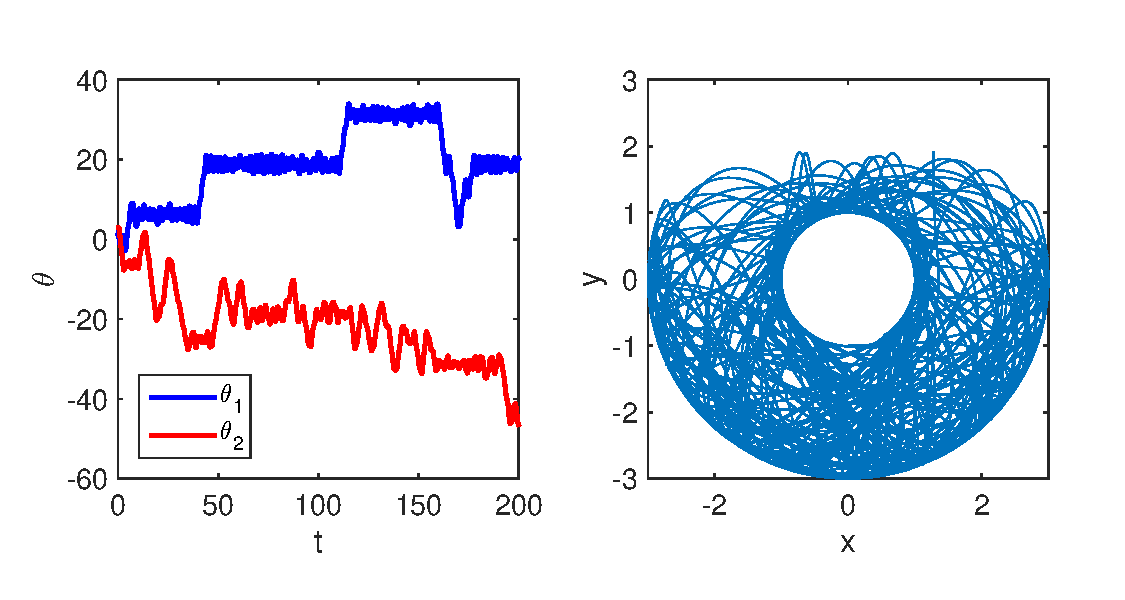
\includegraphics[height=2.5in]{05.ode1/double_pendulum.pdf}
\caption{Chaotic motion of a double pendulum.  Left: Two angular coordinates are randomly drifting.  Right: The trajectory of the bottom bob shows chaotic motion.  Parameter values: $m_1=2\, kg$, $m_2=1\, kg$, $L_1=1\, m$, $L_2=2\, m$, $h=0.02$.]}
\label{fig:double_pendulum}
\end{figure}

\bigskip
\exercise Try to find a regular motion with low energy (small amplitude oscillation).  

%%%
%%% Driven system should be added tothis section.
%%% 

\newpage
\section{Problems}

\begin{enumerate}[labelwidth=0.5cm,labelindent=0cm,leftmargin=*,label=\bfseries \thechapter.\arabic*,align=left]
\item \textbf{Vanishing Friction}~~
A particle of mass $m=1\, kg$ is initially moving freely at velocity $v_0=10\, m/s$.  At $t=0$, a frictional force
\begin{equation}
-\gamma_0\, \me^{-t/\tau}\, v
\end{equation}
is applied, where the friction coefficient is $\gamma_0=0.1\, kg/s$ and the decay constant $\tau = 2s$. Find the velocity $v(t)$ up to $t=10\tau$ using 2nd and 4th order Runge-Kutta methods and estimate the velocity of the particle at $t>>\tau$. Compare the results with the exact solution 
\begin{equation}
v(t) = v_0 \exp \left [ - \frac{\gamma_0 \tau}{m} \left (1-\me^{-t/\tau} \right ) \right ]\, .
\end{equation}


\item  \textbf{FitzHugh-Nagumo Model of Neuron}~~
When electric current stimulate a neuron, the membrane potential generates a spike or train of spikes. A simple mathematical model for such an \emph{excitable media} or \emph{relaxation oscillation} is given by the FitzHugh-Nagumo model\cite{FitzHugh-Nagumo}:
\begin{subequations}
\begin{eqnarray}
\dot{v} &=& v - \frac{1}{3}v^3 - w + I \\
\dot{w} &=& a (v + b - c w)
\end{eqnarray}
\end{subequations}
where $v$ is the membrane potential, $w$ a recovery variable which activate the outgoing current. $I$ is the incoming current which controls the dynamics. Typical parameter values are $a=0.08$, $b=0.7$, $c=0.8$.  Find critical $I$ above which the neuron is excited (the membrane potential periodically oscillates).

\item \textbf{Spring Pendulum}~~
Consider a pendulum consisting of a bob of mass $m$ and a spring (massless) of natural frequency $\omega_0$ and natural length $L_0$.\cite{spring_pendulum}
(See Fig \ref{fig:spring_pendulum}.)  Unlike regular pendulum, length $L$ is a dynamical variable as well as angle $\theta$.  The equations of motion are
\begin{subequations}
\begin{eqnarray}
\ddot{L} &=& L \dot{\theta}^2 - \omega_0^2 (L-L_0) + g \cos\theta \\
L \ddot{\theta} &=& - 2 \dot{L} \dot{\theta} - g \sin\theta
\end{eqnarray}
\end{subequations}

Using $L_0$ and $\omega_0^{-1}$ as units for length and time, respectively, the equations of motion are simplified to
\begin{subequations}
\begin{eqnarray}
\ddot{L} &=& L \dot{\theta}^2 - (L-1) + a \cos\theta \\
L \ddot{\theta} &=& - 2 \dot{L} \dot{\theta} - a \sin\theta
\end{eqnarray}
where $a=\displaystyle\frac{g}{L_0 \omega_0^2}$.  Find trajectories of the bob for various different values of $a$.
\end{subequations}


\begin{figure}
\center
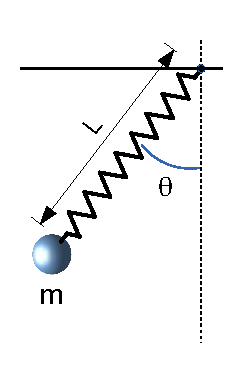
\includegraphics[width=1.2in]{05.ode1/spring-pendulum.pdf}
\caption{A spring pendulum for Problem \ref{ch:ode1}.3.}
\label{fig:spring_pendulum}
\end{figure}
\end{enumerate}

\newpage
\section*{MATLAB Source Codes}
\addcontentsline{toc}{section}{\protect\numberline{}MATLAB Source Codes}

\bigskip
\noindent
\program
\label{prog:freefalling1}

\footnotesize
\begin{verbatim}
%**************************************************************************
%*     Example 5.1                                                        *
%*     filename: ch05pr01.m                                               *
%*     program listing number: 5.1                                        *
%*                                                                        *
%*     This program solves Newton equation for a falling object           *
%*     using Euler and predictor-corrector methods.                       *
%*        m = mass of the object                                          *
%*        g = acceleration due to gravity                                 *
%*        gamma = frictional coefficient                                  *
%*                                                                        *
%*     Programed by Ryoichi Kawai for Computational Physics Course        *
%*     Revised on 01/07/2014.                                             *
%**************************************************************************
clear all;

% system parameters
gamma=1.0;
g=9.8;
m=1.0;

% intial condition
v_ex(1)=0.0;
v_eu(1)=0.0;
v_pc(1)=0.0;
t(1)=0.0;

% integration parameters
tmax=10; % maximum time
N=1000;  % maximum steps
h=tmax/N;% time step

for i=1:N-1
    t(i+1)=t(i)+h;  % time increment
    
    % Euler method
    F_eu=-gamma*v_eu(i)/m-g; 
    v_eu(i+1)=v_eu(i)+F_eu*h;
    
    % Predictor-Corrector method
    F_pc=-gamma*v_pc(i)/m-g;
    v_pc(i+1)=v_pc(i)+F_pc*h;  % predictor
    F_pc =-gamma/m*(v_pc(i)+v_pc(i+1))/2-g;
    v_pc(i+1)=v_pc(i)+F_pc*h;  % corrector
    
    % Exact solution
    v_ex(i+1)=m*g/gamma*(exp(-gamma*t(i+1))-1);
end

subplot(1,2,1);
q=plot(t,v_eu,t,v_pc,t,v_ex);
xlabel('t','fontsize',14);
ylabel('v(t)','fontsize',14);
set(q(1),'Color','blue','Linewidth',2);
set(q(2),'Color','red','Linewidth',2);
set(q(3),'Color','black','Linewidth',2)
legend(q,{'Euler','Predictor-Corrector','Exact'});
legend(q,'Location','NorthEast');

subplot(1,2,2);
% Plot the absolute errors
p=semilogy(t,abs(v_eu-v_ex),t,abs(v_pc-v_ex));

% Plotting options
xlabel('t','fontsize',14);
ylabel('absolute error','fontsize',14);
set(p(1),'Color','blue','Linewidth',2);
set(p(2),'Color','red','Linewidth',2);
legend(p,{'Euler','Predictor-Corrector'});
legend(p,'Location','SouthWest');
\end{verbatim}
\normalsize

\ruleend

\bigskip
\noindent
\program
\label{prog:freefalling2}

\footnotesize
\begin{verbatim}
%**************************************************************************
%*     Example 5.2                                                        *
%*     filename: ch05pr02.m                                               *
%*     program listing number: 5.2                                        *
%*                                                                        *
%*     This program solves Newton equation for a falling object           *
%*     using Runge-Kutta 2nd and 4th order methods.                       *
%*        m = mass of the object                                          *
%*        g = acceleration due to gravity                                 *
%*        gamma = frictional coefficient                                  *
%*                                                                        *
%*     Programed by Ryoichi Kawai for Computational Physics Course        *
%*     Revised on 01/07/2014.                                             *
%**************************************************************************
clear all;

% system parameters
gamma=1.0;
g=9.8;
m=1.0;

% intial condition
v_rk2(1)=0.0;
v_rk4(1)=0.0;
v_pc(1)=0.0;
t(1)=0.0;

% integration parameters
tmax=10; % maximum time
N=1000;  % maximum steps
h=tmax/N;% time step

for i=1:N-1
    t(i+1)=t(i)+h;  % time increment
    
    % Runge-Kutta 2nd order
    k1=-gamma*v_rk2(i)/m-g; 
    v_mid=v_rk2(i)+k1*h/2;
    
    k2=-gamma*v_mid/m-g;
    v_rk2(i+1)=v_rk2(i)+k2*h;
    
    % RUnge-Kutta 4th order
    k1=-gamma*v_rk4(i)/m-g; 
    v_mid=v_rk4(i)+k1*h/2;
    
    k2=-gamma*v_mid/m-g;
    v_mid=v_rk4(i)+k2*h/2;

    k3=-gamma*v_mid/m-g;
    v_end=v_rk4(i)+k3*h;
    
    k4=-gamma*v_end/m-g;
    v_rk4(i+1)=v_rk4(i)+h/6*(k1+2*(k2+k3)+k4);
        
    % Exact solution
    v_ex(i+1)=m*g/gamma*(exp(-gamma*t(i+1))-1);
end

subplot(1,2,1);
q=plot(t,v_rk2,t,v_rk4,t,v_ex);
xlabel('t','fontsize',14);
ylabel('v(t)','fontsize',14);
set(q(1),'Color','blue','Linewidth',2);
set(q(2),'Color','red','Linewidth',2);
set(q(3),'Color','black','Linewidth',2)
legend(q,{'RK2','RK4','Exact'});
legend(q,'Location','NorthEast');

subplot(1,2,2);
% Plot the absolute errors
p=semilogy(t,abs(v_rk2-v_ex),t,abs(v_rk4-v_ex));

% Plotting options
xlabel('t','fontsize',14);
ylabel('absolute error','fontsize',14);
set(p(1),'Color','blue','Linewidth',2);
set(p(2),'Color','red','Linewidth',2);
legend(p,{'RK2','RK4'});
legend(p,'Location','SouthWest');
\end{verbatim}
\normalsize

\ruleend

\bigskip
\noindent
\program
\label{prog:freefalling3}

\footnotesize
\begin{verbatim}
%**************************************************************************
%*     Example 5.3                                                        *
%*     filename: ch05pr03.m                                               *
%*     program listing number: 5.3                                        *
%*                                                                        *
%*     This program solves Newton equation for a falling object           *
%*     using the Runge-Kutta-Fehlberg method.                             *
%*        m = mass of the object                                          *
%*        g = acceleration due to gravity                                 *
%*        gamma = frictional coefficient                                  *
%*                                                                        *
%*     Programed by Ryoichi Kawai for Computational Physics Course        *
%*     Revised on 01/30/2018.                                             *
%**************************************************************************
clear all;

% system parameters
gamma=1.0;
g=9.8;
m=1.0;
% time span
tspan=[0,10]; 
% initial condition
y0=0;
% relative tolerence
rtol=1e-5;

% define the right hand side
f = @(t,v) -gamma*v - m*g;

% use RK45 method
opts=odeset('RelTol',rtol);
[t,v]=ode45(f,tspan,y0,opts);

% exact solution
v_ex = m*g/gamma * (exp(-gamma*t)-1);

subplot(1,2,1);
q=plot(t,v,'o',t,v_ex,'-',t,t*0,'o');
xlabel('t','fontsize',14);
ylabel('v(t)','fontsize',14);
set(q(1),'Color','red','Linewidth',2);
set(q(2),'Color','black','Linewidth',2);
set(q(3),'Color','blue');
legend(q,'RK45','Exact','time step')
legend(q,'Location','East');
hold off

subplot(1,2,2);
% Plot the absolute errors
p=semilogy(t,abs(v-v_ex));

% Plotting options
xlabel('t','fontsize',14);
ylabel('absolute error','fontsize',14);
set(p(1),'Color','blue','Linewidth',2);
\end{verbatim}
\normalsize
\ruleend

\bigskip
\noindent
\program
\label{prog:twocars}

\footnotesize
\begin{verbatim}
%**************************************************************************
%*     Example 5.4                                                        *
%*     filename: ch05pr04.m                                               *
%*     program listing number: 5.4                                        *
%*                                                                        *
%*     This program solves Newton equation for interacting two cars       *
%*     using Runge-Kutta 2nd order methods.                               *
%*                                                                        *
%*     Programed by Ryoichi Kawai for Computational Physics Course        *
%*     Revised on 01/07/2014.                                             *
%**************************************************************************
clear all;

% Control parameters
tmax=8; N=400; h=tmax/N;

% initial conditions
v1(1)=1.2; v2(1)=1.0; t(1)=0;

% 2nd-order Runge-Kutta method
for n=1:N-1
    t(n+1) = t(1)+n*h;
    k1 =   v2(n)-v1(n);
    l1 = -(v2(n)-v1(n));
    mid1 = v1(n)+k1*h/2;
    mid2 = v2(n)+l1*h/2;
    k2 =   mid2-mid1;
    l2 = -(mid2-mid1);
    v1(n+1)=v1(n)+k2*h;
    v2(n+1)=v2(n)+l2*h;
end

subplot(1,2,1); 
p=plot(t,v1,t,v2);
xlabel('t');
ylabel(texlabel('velocity'));
set(p(1),'Color','blue','Linewidth',2);
set(p(2),'Color','red','Linewidth',2);
legend(p,{texlabel('v_1'),texlabel('v_2')});
legend(p,'Location','SouthEast');

subplot(1,2,2);
q=plot(t,v1-v2);
xlabel('t');
ylabel(texlabel('v_1-v_2'));
set(q,'Linewidth',2);
\end{verbatim}
\normalsize

\ruleend

\bigskip
\noindent
\program
\label{prog:harmonic_oscillator1}

\footnotesize
\begin{verbatim}
%**************************************************************************
%*     Example 5.5                                                        *
%*     filename: ch05pr05.m                                               *
%*     program listing number: 5.5                                        *
%*                                                                        *
%*     This program solves Newton equation for simple harmonic oscillator *
%*     using Runge-Kutta 4th order methods.                               *
%*                                                                        *
%*     Programed by Ryoichi Kawai for Computational Physics Course        *
%*     Revised on 01/07/2014.                                             *
%**************************************************************************
clear all;

% system parameter
omega=1;

% initial conditions
x(1)=1;
v(1)=0;
t(1)=0;
x_ex(1)=cos(0);

% control parameters
tmax=8*pi/omega;
N=500;
h=tmax/N

for n=1:N-1
    % 4th-order Runge-Kutta
    kv1=-omega^2*x(n);
    kx1=v(n);
    
    v_mid = v(n)+kv1*h/2;
    x_mid = x(n)+kx1*h/2;
    kv2 = -omega^2*x_mid;
    kx2 = v_mid;
      
    v_mid = v(n)+kv2*h/2;
    x_mid = x(n)+kx2*h/2;
    kv3 = -omega^2*x_mid;
    kx3 = v_mid;

    v_end = v(n)+kv3*h;
    x_end = x(n)+kx3*h;
    kv4 = -omega^2*x_end;
    kx4 = v_end;
    
    v(n+1)=v(n)+(kv1+2*(kv2+kv3)+kv4)*h/6;
    x(n+1)=x(n)+(kx1+2*(kx2+kx3)+kx4)*h/6;
    t(n+1)=t(1)+n*h;
    
    % exact soution
    x_ex(n+1)=cos(omega*t(n+1));
end

% plot trajectories
subplot(1,2,1);
q=plot(t,x,'o',t,x_ex);
xlabel('t');
ylabel('displacement');
set(q(1),'Color','blue','Linewidth',2);
set(q(2),'Color','red','Linewidth',1);
legend(q,{'RK4','Exact'});
legend(q,'Location','East');

% plot absolute error
subplot(1,2,2);
p=semilogy(t,abs(x-x_ex));
xlabel('t');
ylabel('absolute error');
set(p,'Color','blue','Linewidth',2);
\end{verbatim}
\normalsize


\ruleend

\bigskip
\noindent
\program
\label{prog:harmonic_oscillator2}

\footnotesize
\begin{verbatim}
%**************************************************************************
%*     Example 5.6                                                        *
%*     filename: ch05pr06.m                                               *
%*     program listing number: 5.6                                        *
%*                                                                        *
%*     This program solves Newton equation for simple harmonic oscillator *
%*     using Verlet method.                                               *
%*                                                                        *
%*     Programed by Ryoichi Kawai for Computational Physics Course        *
%*     Revised on 01/07/2014.                                             *
%**************************************************************************
clear all;

% system parameter
omega=1;

% initial conditions
x(1)=1;
v(1)=0;
t(1)=0;
x_ex(1)=cos(0);

% control parameters
tmax=8*pi/omega;
N=500;
h=tmax/N;

% the first Euler step
x(2) = x(1) + v(1)*h - omega^2*x(1)*h^2/2;

for n=2:N-1
    % Verlet method
    x(n+1)=2*x(n)-x(n-1) - omega^2*x(n)*h^2;
    t(n+1)=t(1)+n*h;
   
    % exact soution
    x_ex(n+1)=cos(omega*t(n+1));
end

% plot trajectories
subplot(1,2,1);
q=plot(t,x,'o',t,x_ex);
xlabel('t');
ylabel('displacement');
set(q(1),'Color','blue','Linewidth',2);
set(q(2),'Color','red','Linewidth',1);
legend(q,{'Verlet','Exact'});
legend(q,'Location','East');

% plot absolute error
subplot(1,2,2);
p=semilogy(t,abs(x-x_ex));
xlabel('t');
ylabel('absolute error');
set(p,'Color','blue','Linewidth',2);
\end{verbatim}
\normalsize



\ruleend

\bigskip
\noindent
\program
\label{prog:brusselator}

\footnotesize
\begin{verbatim}
%**************************************************************************
%*     Section 5.5.1                                                        *
%*     filename: ch05pr07.m                                               *
%*     program listing number: 5.7                                        *
%*                                                                        *
%*     This program solves the Brusselator model                          *
%*     using Runge-Kutta 4th order methods.                               *
%*                                                                        *
%*     Programed by Ryoichi Kawai for Computational Physics Course        *
%*     Revised on 01/07/2014.                                             *
%**************************************************************************
clear all;

% fixed parameter
a=1;

% control parameter
b=input('Enter value for b [1.5-2.5] =');

%initial conditions
x(1)=1;
y(1)=1;
t(1)=0;

% duration 
tmax=100;

% number of integration steps
N=2000;

% step size
h=tmax/N;

for n=1:N-1
    % 4th-order Runge-Kutta
    kx1=a-(b+1)*x(n)+x(n)^2*y(n);
    ky1=b*x(n)-x(n)^2*y(n);
    
    x_mid = x(n)+kx1*h/2;
    y_mid = y(n)+ky1*h/2;
    kx2 = a - (b+1)*x_mid+x_mid^2*y_mid;
    ky2 = b*x_mid-x_mid^2*y_mid;
      
    x_mid = x(n)+kx2*h/2;
    y_mid = y(n)+ky2*h/2;
    kx3 = a - (b+1)*x_mid+x_mid^2*y_mid;
    ky3 = b*x_mid-x_mid^2*y_mid;

    x_end = x(n)+kx3*h;
    y_end = y(n)+ky3*h;
    kx4 = a - (b+1)*x_end+x_end^2*y_end;
    ky4 = b*x_end-x_end^2*y_end;
    
    x(n+1)=x(n)+(kx1+2*(kx2+kx3)+kx4)*h/6;
    y(n+1)=y(n)+(ky1+2*(ky2+ky3)+ky4)*h/6;
    t(n+1)=t(1)+n*h;
end

% plot individual trajectories
subplot(1,2,1);
p=plot(t,x,t,y);
xlabel('t');
ylabel('concentration');
set(p(1),'Color','blue','Linewidth',2);
set(p(2),'Color','red','Linewidth',2);
legend(p,{'x','y'});
legend(p,'Location','SouthEast');

% plot phase trajectory
subplot(1,2,2);
q=plot(x,y);
xlabel('x');
ylabel('y');
set(q(1),'color','blue');
\end{verbatim}
\normalsize


\ruleend

\bigskip
\noindent
\program
\label{prog:maxwell-bloch}

\footnotesize
\begin{verbatim}
%**************************************************************************
%*     Section 5.5.2                                                      *
%*     filename: ch05pr08.m                                               *
%*     program listing number: 5.8                                        *
%*                                                                        *
%*     This program solves the Maxwell-Bloch model of laser dynamics      *
%*     using Runge-Kutta 2nd order methods.                               *
%*                                                                        *
%*     Programed by Ryoichi Kawai for Computational Physics Course        *
%*     Revised on 01/07/2014.                                             *
%**************************************************************************
clear all;

% system parametes uncomment ONLY the desired set
%Type A
%gamma1=0.1; gamma2=2; gamma3=3; c1=0.25; c2=0.2; c3=1;
%Type B
%gamma1=0.1; gamma2=10; gamma3=0.25; c1=1; c2=0.5; c3=1;
%Type C 
gamma1=1; gamma2=0.1; gamma3=0.25; c1=1; c2=0.1; c3=1;

lambda=input('Enter a value for lambda = ');

% Control parameters
tmax=500; N=5000; h=tmax/N;

% initial conditions
E(1)=1.0; P(1)=1.0; D(1)=1.0; t(1)=0;

% 2nd-order Runge-Kutta method
for n=1:N-1
    t(n+1)=t(1)+n*h;
    FE_n=-gamma1*E(n)+c1*P(n);
    FP_n=-gamma2*P(n)+c2*E(n)*D(n);
    FD_n=-gamma3*(D(n)-lambda)-c3*E(n)*P(n);
    E_mid = E(n)+FE_n*h/2;
    P_mid = P(n)+FP_n*h/2;
    D_mid = D(n)+FD_n*h/2;
    FE_mid=-gamma1*E_mid+c1*P_mid;
    FP_mid=-gamma2*P_mid+c2*E_mid*D_mid;
    FD_mid=-gamma3*(D_mid-lambda)-c3*E_mid*P_mid;
    E(n+1)=E(n)+FE_mid*h;
    P(n+1)=P(n)+FP_mid*h;
    D(n+1)=D(n)+FD_mid*h;
end

% plot the dynamics of E
subplot(1,2,1);
plot(t,E);
xlabel('t');
ylabel('E(t)');

% plot 3D phase trajectory
subplot(1,2,2);
plot3(E,D,P);
xlabel('E');
ylabel('D');
zlabel('P');
grid on
\end{verbatim}
\normalsize

\ruleend

\bigskip
\noindent
\program
\label{prog:kuramoto}

\footnotesize
\begin{verbatim}
%**************************************************************************
%*     Section 5.5.3                                                      *
%*     filename: ch05pr09.m                                               *
%*     program listing number: 5.9                                        *
%*                                                                        *
%*     This program solves the synchronization of two phase oscillators   *
%*     using 2nd-order Runge-Kutta methods.                               *
%*                                                                        *
%*     Programed by Ryoichi Kawai for Computational Physics Course        *
%*     Revised on 01/07/2014.                                             *
%**************************************************************************
clear all;

omega1=1.0;  omega2=1.2;

% Control parameters
tmax=20; N=2000; h=tmax/N;

% initial conditions
theta1(1)=pi; theta2(1)=0; t(1)=0;

% 2nd-order Runge-Kutta method
for n=1:N-1
    t(n+1) = t(1)+n*h;
    k1 = omega1 + sin(theta2(n)-theta1(n));
    l1 = omega2 - sin(theta2(n)-theta1(n));
    mid1 = theta1(n)+k1*h/2;
    mid2 = theta2(n)+l1*h/2;
    k2 = omega1 + sin(mid2-mid1);
    l2 = omega2 - sin(mid2-mid1);
    theta1(n+1)=theta1(n)+k2*h;
    theta2(n+1)=theta2(n)+l2*h;
end

% plot the trajectories of oscillators
subplot(1,2,1); 
p=plot(t,sin(theta1),t,sin(theta2));
xlabel('t');
ylabel(texlabel('sin theta'));
set(p(1),'Color','blue','Linewidth',2);
set(p(2),'Color','red','Linewidth',2);
legend(p,{texlabel('theta_1'),texlabel('theta_2')});
legend(p,'Location','SouthEast');

% plot the phase difference
subplot(1,2,2);
q=plot(t,theta1-theta2);
xlabel('t');
ylabel(texlabel('theta_1-theta_2'));
set(q,'Linewidth',2);
\end{verbatim}
\normalsize


\ruleend

\bigskip
\noindent
\program\label{prog:period}

\footnotesize
\begin{verbatim}
%**************************************************************************
%*     Section 5.5.4                                                      *
%*     filename: ch05pr10.m                                               *
%*     program listing number: 5.10                                       *
%*                                                                        *
%*     This program solves Newton equation for simple harmonic oscillator *
%*     using Runge-Kutta 4th order methods.  Then, it determines the      *
%*     period of the oscillation.                                         *
%*                                                                        *
%*     Programed by Ryoichi Kawai for Computational Physics Course        *
%*     Revised on 01/07/2014.                                             *
%**************************************************************************
clear all;

% system parameter
omega=1; mass=1; spring_k=mass*omega^2;

% initial conditions
E=1; 
t(1)=0; x(1)=0;
v(1)=sqrt(2*(E-spring_k*x(1)^2/2)/mass);

% control parameters
h=0.01;
N=0; Nmax=10;
n=1;

% the first Euler step
x(2) = x(1) + v(1)*h - omega^2*x(1)*h^2/2;

while N<Nmax
    n=n+1;
    % Verlet method
    x(n+1)=2*x(n)-x(n-1) - omega^2 * x(n) * h^2;
    v(n) = (x(n+1)-x(n-1))/(2*h);
    t(n+1)=t(1)+n*h;
    
    % Check if it returned to the tarting point
    if x(n+1)-x(1)>0 & x(n)-x(1)< 0 
        N=N+1;
    end
end

% adjustment of the return time
Fn = -omega^2*x(n)/mass;
if Fn>0 
    delta = (-2*(x(n)-x(1)))/(v(n)+sqrt( v(n)^2-2*(x(n)-x(1))*Fn));
else
    delta = (-v(n)-sqrt( v(n)^2-2*(x(n)-x(1))*Fn))/Fn;
end

tau = t(n)+delta;
period = tau/N;

fprintf('Period: Verlet = %7.6f,  Exact = %7.6f \n',period,2*pi);
\end{verbatim}
\normalsize


\ruleend

\bigskip
\noindent
\program
\label{prog:pendulum}

\footnotesize
\begin{verbatim}
%**************************************************************************
%*     Section 5.5.5                                                      *
%*     filename: ch05pr11.m                                               *
%*     program listing number: 5.11                                       *
%*                                                                        *
%*     This program finds the trajectory of a pendulum using              *
%*     Euler and Verlet methods.    Euler method shows its numerical      *
%*     instability and the trajectory diverges.                           *
%*                                                                        *
%*     Programed by Ryoichi Kawai for Computational Physics Course        *
%*     Revised on 01/07/2014.                                             *
%**************************************************************************


% system parameters
mass=1; L=1; g=9.8; Omega=sqrt(g/L); I=mass*L^2;

% initial conditions
theta1(1)=0.5; omega1(1)=0;t(1)=0;
theta2(1)=0.5; omega2(1)=0;
E1(1) = - mass*g*L*cos(theta1(1));
E2(1) = - mass*g*L*cos(theta2(1));

% control parameters
tmax=50; N=5000; h=tmax/N;

% Euler method
for i=1:N-1
    t(i+1)=t(1)+i*h;
    omega1(i+1) = omega1(i) - Omega^2 * sin(theta1(i)) * h;
    theta1(i+1) = theta1(i) + omega1(i)*h;
    E1(i+1) = I/2 * omega1(i+1)^2 - mass*g*L*cos(theta1(i+1));
end

% Verlet method
theta2(2) = theta2(1) + omega2(1)*h- Omega^2 * sin(theta2(1))*h^2/2;
for i=2:N
    theta2(i+1)=2*theta2(i)-theta2(i-1)-Omega^2 * sin(theta2(i))*h^2;
    omega2(i) = (theta2(i+1)-theta2(i-1))/(2*h);
    E2(i)=I/2 * omega2(i)^2 - mass*g*L*cos(theta2(i));
end

subplot(1,2,1);
q=plot(t(1:N),theta1(1:N),t(1:N),theta2(1:N));
xlabel('t');
ylabel(texlabel('theta'));
set(q(1),'Color','blue','Linewidth',2);
set(q(2),'Color','red','Linewidth',2);
legend(q,{'Euler','Verlet'});
legend(q,'Location','SouthWest');

subplot(1,2,2);
p=plot(t(1:N),E1(1:N),t(1:N),E2(1:N));
xlabel('t');
ylabel('Energy');
set(p(1),'Color','blue','Linewidth',2);
set(p(2),'Color','red','Linewidth',2);
legend(p,{'Euler','Verlet'});
legend(p,'Location','NorthWest');
\end{verbatim}
\normalsize


\ruleend

\bigskip
\noindent
\program
\label{prog:scattering2}

\footnotesize
\begin{verbatim}
%**************************************************************************
%*     Section 5.5.6                                                      *
%*     filename: ch05pr12.m                                               *
%*     program listing number: 5.12                                       *
%*                                                                        *
%*     This program calculate the trajectory of a particle scattered by   *
%*     Yukawa potential using he Valet method.                            *
%*                                                                        *
%*     Programed by Ryoichi Kawai for Computational Physics Course        *
%*     Revised on 01/07/2014.                                             *
%**************************************************************************
lear all;

E=input('Enter Energy =');

% control parameter
bmax=3;
N=10;
db=bmax/N;
h=0.01;

subplot(1,2,1);

for i=1:2*N+1
    
    % set impact parameter
    b(i)=db*(i-N-1);
    
    % initial conditions
    x(1)=-10; y(1)=b(i); vx(1)=sqrt(2*E); vy(1)=0;
    
    % first Euler step
    r = sqrt(x(1)^2+y(1)^2);
    Fx=x(1)/r^2 * (1/r+1) * exp(-r);
    Fy=y(1)/r^2 * (1/r+1) * exp(-r);
    x(2)=x(1)+vx(1)*h+Fx*h^2/2;
    y(2)=y(1)+vy(1)*h+Fy*h^2/2;
    
    % Verlet method
    n=2;
    while abs(x(n))<10
        r = sqrt(x(n)^2+y(n)^2);
        Fx=x(n)/r^2 * (1/r+1) * exp(-r);
        Fy=y(n)/r^2 * (1/r+1) * exp(-r);
        x(n+1)=2*x(n)-x(n-1)+Fx*h^2;
        y(n+1)=2*y(n)-y(n-1)+Fy*h^2;
        n=n+1;
    end
    
    % final velocity
    vfx=(x(n)-x(n-2))/(2*h);
    vfy=(y(n)-y(n-2))/(2*h);
    
    % scattering angle
    theta(i) = acos((vx(1)*vfx+vy(1)*vfy)/(2*E));
    
    % plot the trajctory
    plot(x(1:n),y(1:n));
    hold on
end

% draw a target atom
p=plot(0,0,'o');
set(p,'Color','red','Linewidth',3);
hold off

axis([-10,10,-10,10]);
xlabel('x');
ylabel('y');

% plot scattering angle
subplot(1,2,2);
q=plot(b,theta);
xlabel('Impact Parameter');
ylabel('Scattering Angle theta');
set(q,'Linewidth',2);
\end{verbatim}
\normalsize


\ruleend

\bigskip
\noindent
\program
\label{prog:double_pendulum}

\footnotesize
\begin{verbatim}
%**************************************************************************
%*     Section 5.5.7                                                      *
%*     filename: ch05pr13.m                                               *
%*     program listing number: 5.13                                       *
%*                                                                        *
%*     This program calculate the trajectory of a double pendulum by      *
%*     the 4th order Runge-Kutta method.                                  *
%*                                                                        *
%*     Programed by Ryoichi Kawai for Computational Physics Course        *
%*     Revised on 01/07/2014.                                             *
%**************************************************************************
clear all;



% system parameters 
global m1 m2 L1 L2 g
m1=2; m2=1; L1=1; L2=2; g=9.8;

% initial conditions
q1(1)=1.5;
q2(1)=3.0;
w1(1)=0;
w2(1)=0.0;
t(1)=0;
V = -(m1+m2)*g*L1*cos(q1(1))-m2*g*L2*cos(q2(1));
T = m1*L1^2*w1(1)^2/2+m2*(L1^2*w1(1)^2+L2^2*w2(1)^2 ...
    +2*L1*L2*w1(1)*w2(1)*cos(q1(1)-q2(1)))/2;
E = T+V;
 
% control parameter
tmax=200;
N=10000;
h=tmax/N;

for n=1:N-1
    % 4th-order Runge-Kutta
    dotw=DP(q1(n),q2(n),w1(n),w2(n));
    kw11=dotw(1);
    kw21=dotw(2);
    kq11=w1(n);
    kq21=w2(n);
    
    w1m = w1(n)+kw11*h/2;
    w2m = w2(n)+kw21*h/2;
    q1m = q1(n)+kq11*h/2;
    q2m = q2(n)+kq21*h/2;
    
    dotw=DP(q1m,q2m,w1m,w2m);
    kw12 = dotw(1);
    kw22 = dotw(2);
    kq12 = w1m;
    kq22 = w2m;
    
    w1m = w1(n)+kw12*h/2;
    w2m = w2(n)+kw22*h/2;
    q1m = q1(n)+kq12*h/2;
    q2m = q2(n)+kq22*h/2;

    dotw=DP(q1m,q2m,w1m,w2m);
    kw13 = dotw(1);
    kw23 = dotw(2);
    kq13 = w1m;
    kq23 = w2m;
    
    w1f = w1(n)+kw13*h;
    w2f = w2(n)+kw23*h;
    q1f = q1(n)+kq13*h;
    q2f = q2(n)+kq23*h;
    
    dotw=DP(q1f,q2f,w1f,w2f);
    kw14 = dotw(1);
    kw24 = dotw(2);
    kq14 = w1f;
    kq24 = w2f;
    
    q1(n+1)=q1(n)+(kq11+2*(kq12+kq13)+kq14)*h/6;
    q2(n+1)=q2(n)+(kq21+2*(kq22+kq23)+kq24)*h/6;
    w1(n+1)=w1(n)+(kw11+2*(kw12+kw13)+kw14)*h/6;
    w2(n+1)=w2(n)+(kw21+2*(kw22+kw23)+kw24)*h/6;

    V = -(m1+m2)*g*L1*cos(q1(n+1))-m2*g*L2*cos(q2(n+1));
    T = m1*L1^2*w1(n+1)^2/2+m2*(L1^2*w1(n+1)^2+L2^2*w2(n+1)^2 ...
        +2*L1*L2*w1(n+1)*w2(n+1)*cos(q1(n+1)-q2(n+1)))/2;
    E(n+1)=T+V;
    t(n+1)=t(1)+n*h;
end

% plot angular coordinates
subplot(1,2,1);
p=plot(t,q1,t,q2);
xlabel('t');
ylabel(texlabel('theta'));
set(p(1),'Color','blue','Linewidth',2);
set(p(2),'Color','red','Linewidth',2);
legend(p,texlabel('theta_1'),texlabel('theta_2'));
legend('Location','SouthWest');

% trajectory of the second bob in xy coordiates
subplot(1,2,2);
axis square;
x2=L1*sin(q1)+L2*sin(q2);
y2=-L1*cos(q1)-L2*cos(q2);
plot(x2,y2);
xlabel('x');
ylabel('y');
\end{verbatim}
\normalsize

\section*{Python Source Codes}
\addcontentsline{toc}{section}{\protect\numberline{}Python Source Codes}
\setcounter{program}{0}

\noindent
\program
\footnotesize
\begin{verbatim}
#!/usr/bin/env python3
# -*- coding: utf-8 -*-
"""
%**************************************************************************
%*     Example 5.1                                                        *
%*     filename: ch05pr01.py                                              *
%*     program listing number: 5.1                                        *
%*                                                                        *
%*     This program solves Newton equation for a falling object           *
%*     using Euler and predictor-corrector methods.                       *
%*        m = mass of the object                                          *
%*        g = acceleration due to gravity                                 *
%*        gamma = frictional coefficient                                  *
%*                                                                        *
%*     Programed by Ryoichi Kawai for Computational Physics Course        *
%*     Revised on 01/20/2017.                                             *
%**************************************************************************
"""
import numpy as np
import matplotlib.pyplot as plt

# system parameters
gamma=1.0
g=9.8
m=1.0

# integration parameters
tmax=10  # maximum time
N=1000   # maximum steps
h=tmax/N # time step

# set arrays
v_ex=np.zeros(N+1)
v_eu=np.zeros(N+1)
v_pc=np.zeros(N+1)
t=np.linspace(0,N,N+1)*h

# intial condition
v_ex[0]=0.0
v_eu[0]=0.0
v_pc[0]=0.0

for i in range(0,N):
    # Euler method
    F_eu = -gamma*v_eu[i]/m - g 
    v_eu[i+1] = v_eu[i] + F_eu*h
    
    # Predictor-Corrector method
    F_pc = -gamma*v_pc[i]/m - g
    v_pc[i+1] = v_pc[i] + F_pc*h;  # predictor
    F_pc = -gamma/m*(v_pc[i]+v_pc[i+1])/2 - g
    v_pc[i+1] = v_pc[i] + F_pc*h   # corrector
    
    # Exact solution
    v_ex[i+1] = m*g/gamma*(np.exp(-gamma*t[i+1])-1)

plt.ioff()
plt.figure(figsize=(12,5))

# Plot the solutions
plt.subplot(1,2,1);
plt.plot(t,v_eu,'-b',label='Euler')
plt.plot(t,v_pc,'-r',label='Predictor-Corrector')
plt.plot(t,v_ex,'-k',label='Exact')
plt.xlabel('t')
plt.ylabel('v(t)')
plt.legend(loc=1)

# Plot the absolute errors
plt.subplot(1,2,2)
plt.semilogy(t,abs(v_eu-v_ex),'-b',label='Euler')
plt.semilogy(t,abs(v_pc-v_ex),'-r',label='Predictor-Corrector')

plt.xlabel('t')
plt.ylabel('absolute error')
plt.legend(loc=3)
plt.show()
\end{verbatim}

\normalsize
\ruleend
\bigskip

\noindent
\program
\footnotesize
\begin{verbatim}
#!/usr/bin/env python3
# -*- coding: utf-8 -*-
"""
%**************************************************************************
%*     Example 5.2                                                        *
%*     filename: ch05pr02.m                                               *
%*     program listing number: 5.2                                        *
%*                                                                        *
%*     This program solves Newton equation for a falling object           *
%*     using Runge-Kutta 2nd and 4th order methods.                       *
%*        m = mass of the object                                          *
%*        g = acceleration due to gravity                                 *
%*        gamma = frictional coefficient                                  *
%*                                                                        *
%*     Programed by Ryoichi Kawai for Computational Physics Course        *
%*     Revised on 01/07/2014.                                             *
%**************************************************************************
"""
import numpy as np
import matplotlib.pyplot as plt

# system parameters
gamma=1.0
g=9.8
m=1.0

# integration parameters
tmax=10  # maximum time
N=1000   # maximum steps
h=tmax/N # time step

# set arrays
v_rk45=np.zeros(N+1)
v_ex=np.zeros(N+1)
t=

for i in range(0,N):
    
    # Runge-Kutta 2nd order
    k1 = -gamma*v_rk2[i]/m - g
    v_mid = v_rk2[i] + k1*h/2.0
    k2 = -gamma*v_mid/m - g
    v_rk2[i+1] = v_rk2[i] + k2*h
    
    # RUnge-Kutta 4th order
    k1 = -gamma*v_rk4[i]/m - g
    v_mid = v_rk4[i] + k1*h/2.0
    k2 = -gamma*v_mid/m - g
    v_mid = v_rk4[i] + k2*h/2
    k3 = -gamma*v_mid/m - g
    v_end = v_rk4[i] + k3*h    
    k4 = -gamma*v_end/m - g
    v_rk4[i+1] = v_rk4[i] + (k1+2*(k2+k3)+k4)*h/6.0
        
    # Exact solution
    v_ex[i+1] = m*g/gamma*(np.exp(-gamma*t[i+1])-1)
    
plt.ioff()
plt.figure(figsize=(12,5))

# Plot the solutions
plt.subplot(1,2,1);
plt.plot(t,v_rk2,'-b',label='RK2')
plt.plot(t,v_rk4,'-r',label='RK4')
plt.plot(t,v_ex,'-k',label='Exact')
plt.xlabel('t')
plt.ylabel('v(t)')
plt.legend(loc=1)

# Plot the absolute errors
plt.subplot(1,2,2)
plt.semilogy(t,abs(v_rk2-v_ex),'-b',label='RK2')
plt.semilogy(t,abs(v_rk4-v_ex),'-r',label='RK4')

plt.xlabel('t')
plt.ylabel('absolute error')
plt.legend(loc=3)
plt.show()
\end{verbatim}

\normalsize
\ruleend
\bigskip
\noindent
\program
\footnotesize
\begin{verbatim}
#!/usr/bin/env python3
# -*- coding: utf-8 -*-
"""
%**************************************************************************
%*     Example 5.3                                                        *
%*     filename: ch05pr03.py                                              *
%*     program listing number: 5.3                                        *
%*                                                                        *
%*     This program solves Newton equation for a falling object           *
%*     using the Runge-Kutta-Fehlberg method.                             *
%*        m = mass of the object                                          *
%*        g = acceleration due to gravity                                 *
%*        gamma = frictional coefficient                                  *
%*                                                                        *
%*     Programed by Ryoichi Kawai for Computational Physics Course        *
%*     Revised on 01/30/2018.                                             *
%**************************************************************************
"""

import numpy as np
from scipy.integrate import solve_ivp
import matplotlib.pyplot as plt


# define the right hand side of ODE   
def func(t,v):
return -gamma*v-m*g

if __name__ == "__main__":

# system parameters
gamma=1.0
m=1.0
g=9.8
# time span
tspan=[0,10]
# initial condition (must be ndarray)
y0=[0]
#relative tolerence
rtol=1e-5

# use RK45 method
sol=solve_ivp(func,tspan,y0,method='RK45',rtol=rtol)
# save the results
t=sol.t
v=list(sol.y.flat)

# exact solution
v_ex=m*g/gamma * (np.exp(-gamma*t)-1)

plt.ioff()
plt.figure(figsize=(12,5))

plt.subplot(1,2,1) 
plt.plot(t,v,'or',label="RK45")
plt.plot(t,v_ex,'-k',label="Exact")
plt.plot(t,t*0,'ob',label="Time step")
plt.xlabel('t')
plt.ylabel('velocity')
plt.legend(loc=0)

plt.subplot(1,2,2)
plt.semilogy(t,abs(v-v_ex),'-k')
plt.xlabel('t')
plt.ylabel("absolute error")
plt.show()
\end{verbatim}

\normalsize
\ruleend

\bigskip
\noindent
\program
\footnotesize
\begin{verbatim}
#!/usr/bin/env python3
# -*- coding: utf-8 -*-
"""
%**************************************************************************
%*     Example 5.4                                                        *
%*     filename: ch05pr04.py                                              *
%*     program listing number: 5.4                                        *
%*                                                                        *
%*     This program solves Newton equation for interacting two cars       *
%*     using Runge-Kutta 2nd order methods.                               *
%*                                                                        *
%*     Programed by Ryoichi Kawai for Computational Physics Course        *
%*     Revised on 01/22/2017.                                             *
%**************************************************************************
"""
import numpy as np
import matplotlib.pyplot as plt

# Control parameters
tmax=8; N=400; h=tmax/N;

t=np.linspace(0,tmax,N+1)
v1=np.zeros(N+1)
v2=np.zeros(N+1)

#initial conditions
v1[0]=1.2; v2[0]=1.0

# 2nd-order Runge-Kutta method
for n in range(0,N):
    k1 =   v2[n]-v1[n]
    l1 = -(v2[n]-v1[n])
    mid1 = v1[n]+k1*h/2
    mid2 = v2[n]+l1*h/2
    k2 =   mid2-mid1
    l2 = -(mid2-mid1)
    v1[n+1]=v1[n]+k2*h
    v2[n+1]=v2[n]+l2*h

plt.ioff()
plt.figure(figsize=(12,5))

plt.subplot(1,2,1) 
plt.plot(t,v1,'-b',label="$v_1$")
plt.plot(t,v2,'-r',label="$v_2$")
plt.xlabel('t')
plt.ylabel('velocity')
plt.legend(loc=1)

plt.subplot(1,2,2)
plt.plot(t,v1-v2,'-k')
plt.xlabel('t')
plt.ylabel("$v_1-v_2$")
plt.show()
\end{verbatim}

\normalsize
\ruleend

\bigskip
\noindent
\program
\footnotesize
\begin{verbatim}
#!/usr/bin/env python3
# -*- coding: utf-8 -*-
"""
%**************************************************************************
%*     Example 5.5                                                        *
%*     filename: ch05pr05.py                                              *
%*     program listing number: 5.5                                        *
%*                                                                        *
%*     This program solves Newton equation for simple harmonic oscillator *
%*     using Runge-Kutta 4th order methods.                               *
%*                                                                        *
%*     Programed by Ryoichi Kawai for Computational Physics Course        *
%*     Revised on 01/22/2017.                                             *
%**************************************************************************
"""
import numpy as np
import matplotlib.pyplot as plt

# system parameter
omega=1.0

# control parameters
tmax=8.0*np.pi/omega
N=500
h=tmax/N

t=np.linspace(0,tmax,N+1)
x=np.zeros(N+1)
v=np.zeros(N+1)

# exact soution
x_ex=np.cos(omega*t)

# initial conditions
x[0]=1.0
v[0]=0.0

for n in range(0,N):
    # 4th-order Runge-Kutta
    kv1=-omega**2*x[n];
    kx1=v[n];
    
    v_mid = v[n]+kv1*h/2.0
    x_mid = x[n]+kx1*h/2.0
    kv2 = -omega**2*x_mid
    kx2 = v_mid
      
    v_mid = v[n]+kv2*h/2.0
    x_mid = x[n]+kx2*h/2.0
    kv3 = -omega**2*x_mid
    kx3 = v_mid

    v_end = v[n]+kv3*h
    x_end = x[n]+kx3*h
    kv4 = -omega**2*x_end
    kx4 = v_end
    
    v[n+1]=v[n]+(kv1+2.0*(kv2+kv3)+kv4)*h/6.0
    x[n+1]=x[n]+(kx1+2.0*(kx2+kx3)+kx4)*h/6.0

# plot trajectories
plt.ioff()
plt.figure(figsize=(12,5))

plt.subplot(1,2,1)
plt.plot(t,x,'ob',label='RK4')
plt.plot(t,x_ex,'-r',label='Exact')
plt.xlabel('t')
plt.ylabel('displacement')
plt.legend(loc=1)

# plot absolute error
plt.subplot(1,2,2)
plt.semilogy(t,abs(x-x_ex),'-k')
plt.xlabel('t');
plt.ylabel('absolute error')
plt.show()
\end{verbatim}

\normalsize
\ruleend

\bigskip
\noindent
\program
\footnotesize
\begin{verbatim}
#!/usr/bin/env python3
# -*- coding: utf-8 -*-
"""
%**************************************************************************
%*     Example 5.6                                                        *
%*     filename: ch05pr06.py                                              *
%*     program listing number: 5.6                                        *
%*                                                                        *
%*     This program solves Newton equation for simple harmonic oscillator *
%*     using Verlet method.                                               *
%*                                                                        *
%*     Programed by Ryoichi Kawai for Computational Physics Course        *
%*     Revised on 01/22/2017.                                             *
%**************************************************************************
"""
import numpy as np
import matplotlib.pyplot as plt

# system parameter
omega=1;

# control parameters
tmax=8.0*np.pi/omega
N=500
h=tmax/N

t=np.linspace(0,tmax,N+1)
x=np.zeros(N+1)
v=np.zeros(N+1)

# exact soution
x_ex=np.cos(omega*t)

# initial conditions
x[0]=1.0
v[0]=0.0

# the first Euler step
x[1] = x[0] + v[0]*h - omega**2*x[0]*h**2/2.0

for n in range(1,N):
    # Verlet method
    x[n+1]=2*x[n]-x[n-1] - omega**2*x[n]*h**2;


# plot trajectories
plt.ioff()
plt.figure(figsize=(12,5))

plt.subplot(1,2,1)
plt.plot(t,x,'ob',label='Verlet')
plt.plot(t,x_ex,'-r',label='Exact')
plt.xlabel('t')
plt.ylabel('displacement')
plt.legend(loc=1)

# plot absolute error
plt.subplot(1,2,2)
plt.semilogy(t,abs(x-x_ex),'-k')
plt.xlabel('t');
plt.ylabel('absolute error')
plt.show()
\end{verbatim}

\normalsize
\ruleend

\bigskip
\noindent
\program
\footnotesize
\begin{verbatim}
#!/usr/bin/env python3
# -*- coding: utf-8 -*-
"""
%**************************************************************************
%*     Section 5.5.1                                                      *
%*     filename: ch05pr07.py                                              *
%*     program listing number: 5.7                                        *
%*                                                                        *
%*     This program solves the Brusselator model                          *
%*     using Runge-Kutta 4th order methods.                               *
%*                                                                        *
%*     Programed by Ryoichi Kawai for Computational Physics Course        *
%*     Revised on 01/22/2017.                                             *
%**************************************************************************
"""
import numpy as np
import matplotlib.pyplot as plt

# fixed parameter
a=1.0

# control parameter
b=np.float(input('Enter value for b [1.5-2.5] ='))

# duration 
tmax=100
# number of integration steps
N=2000
# step size
h=tmax/N

t=np.linspace(0,tmax,N+1)
x=np.zeros(N+1)
y=np.zeros(N+1)

#initial conditions
x[0]=1.0
y[0]=1.0

for n in range(0,N):
    # 4th-order Runge-Kutta
    kx1=a-(b+1)*x[n]+x[n]**2*y[n]
    ky1=b*x[n]-x[n]**2*y[n]
    
    x_mid = x[n]+kx1*h/2.0
    y_mid = y[n]+ky1*h/2.0
    kx2 = a - (b+1.0)*x_mid+x_mid**2*y_mid
    ky2 = b*x_mid-x_mid**2*y_mid
      
    x_mid = x[n]+kx2*h/2.0
    y_mid = y[n]+ky2*h/2.0
    kx3 = a - (b+1.0)*x_mid+x_mid**2*y_mid
    ky3 = b*x_mid-x_mid**2*y_mid

    x_end = x[n]+kx3*h
    y_end = y[n]+ky3*h
    kx4 = a - (b+1.0)*x_end+x_end**2*y_end
    ky4 = b*x_end-x_end**2*y_end
    
    x[n+1]=x[n]+(kx1+2.0*(kx2+kx3)+kx4)*h/6.0
    y[n+1]=y[n]+(ky1+2.0*(ky2+ky3)+ky4)*h/6.0

# plot individual trajectories
plt.ioff()
plt.figure(figsize=(12,5))

plt.subplot(1,2,1);
plt.plot(t,x,'-b',label='x')
plt.plot(t,y,'-r',label='y')
plt.xlabel('t');
plt.ylabel('concentration');
plt.legend(loc=1)

# plot phase trajectory
plt.subplot(1,2,2)
plt.plot(x,y,'-b')
plt.xlabel('x')
plt.ylabel('y');
plt.show()
\end{verbatim}

\normalsize
\ruleend

\bigskip
\noindent
\program
\footnotesize
\begin{verbatim}
#!/usr/bin/env python3
# -*- coding: utf-8 -*-
"""
%**************************************************************************
%*     Section 5.5.2                                                      *
%*     filename: ch05pr08.py                                              *
%*     program listing number: 5.8                                        *
%*                                                                        *
%*     This program solves the Maxwell-Bloch model of laser dynamics      *
%*     using Runge-Kutta 4th order methods.                               *
%*                                                                        *
%*     Programed by Ryoichi Kawai for Computational Physics Course        *
%*     Revised on 01/22/2017.                                             *
%**************************************************************************
"""
import numpy as np
import matplotlib.pyplot as plt
from mpl_toolkits.mplot3d import Axes3D

# system parametes uncomment ONLY the desired set
gamma1_set = {0: 0.1, 1: 0.1, 2: 1.0}
gamma2_set = {0: 2.0, 1: 10.0, 2: 0.1}
gamma3_set = {0: 3.0, 1: 0.25, 2: 0.25}
c1_set = {0: 0.25, 1: 1.0, 2: 1.0}
c2_set = {0: 0.2, 1: 0.5, 2: 0.1}
c3_set = {0: 1.0, 1: 1.0, 2: 1.0}

param=np.int(input('Choose a parameter set [0-2] ='))
gamma1=gamma1_set.get(param)
gamma2=gamma2_set.get(param)
gamma3=gamma3_set.get(param)
c1=c1_set.get(param)
c2=c2_set.get(param)
c3=c3_set.get(param)

lam=np.float(input('Enter a value for lambda = '))

# Control parameters
tmax=500; N=5000; h=tmax/N
t=np.linspace(0,tmax,N+1)

E=np.zeros(N+1)
P=np.zeros(N+1)
D=np.zeros(N+1)

# initial conditions
E[0]=1.0; P[0]=1.0; D[0]=1.0

# 2nd-order Runge-Kutta method
for n in range(0,N):
    FE_n=-gamma1*E[n]+c1*P[n]
    FP_n=-gamma2*P[n]+c2*E[n]*D[n]
    FD_n=-gamma3*(D[n]-lam)-c3*E[n]*P[n]
    E_mid = E[n]+FE_n*h/2.0
    P_mid = P[n]+FP_n*h/2.0
    D_mid = D[n]+FD_n*h/2.0
    FE_mid=-gamma1*E_mid+c1*P_mid
    FP_mid=-gamma2*P_mid+c2*E_mid*D_mid
    FD_mid=-gamma3*(D_mid-lam)-c3*E_mid*P_mid
    E[n+1]=E[n]+FE_mid*h
    P[n+1]=P[n]+FP_mid*h
    D[n+1]=D[n]+FD_mid*h


# plot the dynamics of E
plt.ioff()
fig=plt.figure(figsize=(12,5))
ax=fig.add_subplot(1,2,1)
ax.plot(t,E)
ax.set_xlabel('t')
ax.set_ylabel('E(t)')

# plot 3D phase trajectory
ax = fig.add_subplot(1,2,2,projection='3d')
ax.plot(D, E, P)
ax.set_xlabel('D')
ax.set_ylabel('E')
ax.set_zlabel('P')
plt.show()
\end{verbatim}

\normalsize
\ruleend

\newpage
\vfill
\bibliographystyle{unsrt}
\bibliography{compphys}


